%%% -*-LaTeX-*-

\chapter{Results And Discussion}\label{results}
%\section{Finite Element Comparisons}\label{2d_3d_comparison}

To verify the structural-element model, which can only be analyzed with nonlinear geometry, we
compare the displacements of the shell element model to those of the continuum
element model. The displacement BC applied to these models is a 0.01 mm in the
x-direction on surface 3. The first comparison in Figure
\ref{fig:2d_mesh_converge_coarse} shows the two separate models.  The mesh size
of the structural-element model is 12.7 mm. The displacement has been magnified
by 1000 to make clear the deformations. There are apparent disparities between the
displacements of the two models, with the largest being 7\% near the center of
the plate. The mesh size is repeatedly reduced by half until a size of 0.4 mm.
At that mesh size, a percent difference of the displacements falls below 1\%.  

Figure \ref{fig:nl_sload_error} shows the percent error (difference) between the
structural- and 3D solid-element models.  Percent error is computed at 609
points, which are equally spaced out across the model. These points are where the coordinates of the structural element model correspond directly to the coordinates of the 3D solid element model. The distance between the points was approximately the element size of the structural element mesh. The error plotted is the maximum error of the 609 points at
five values of applied x displacement on surface 3.  This BC was chosen for
illustration purposes because it resulted in the largest discrepancies between
the two models.  It is evident that this disparity is due to the eccentricities
in the flanges of the c-channel.

Figure \ref{fig:nl_sload_error} shows a nearly linear relationship between error
and displacement:  the displacement at which error is below 1\% is interpolated
as 0.016 mm. However, to account for possible larger errors when displacements
are combined, the maximum displacement of surface 3 is set at 0.01 mm. A similar
approach is taken for each of the four applied BCs. The results for the maximum allowed
displacement applied to each surface to remain below 1\% error is shown in Table
\ref{tab:max_disps}. 

\section{Sensitivity Analysis}\label{sensitivity_results}

Figure \ref{fig:mps_vs_rstl} shows the relationship between each of the defined
displacement boundary conditions and the maximum principal stress at a single
point at the center of the weld surface.  The results of a Sobol sensitivity
analysis are listed in Table \ref{tab:sobol_indices} as sensitivity indices. We
see that the maximum principal stress is most sensitive to the x-displacement on
surface 4.  The lowest sensitivity index is for x-displacement on surface 3.
However, it has high interaction effects with the other displacement BCs as
evidenced by the larger total effect index, ST. From these results of the sensitivity analysis, to arrive at the 180 different loading conditions we need,
as discussed in section \ref{sensitivity_analysis}, five different displacement
values for the x-displacement on surface 4, four displacement values for the
y-displacement on surfaces 4 and 40, and three different displacement values for
the other two displacement BCs. The 180 different combinations of these BCs will
be our defined BCs for the FRANC3D simulations of crack propagation.

\section{Fracture Analysis}\label{franc_results}

The convergence study discussed in \ref{franc3d} was performed.  Unresolvable errors
occurred within Franc3D in the case where surface 4 is displaced in the
x-direction when the crack growth was too small. Typically, a convergence study
would reduce the size by half at each subsequent step; however, due to the
nature of the re-meshing step in Franc3D, crack size may need to be adjusted to
allow for crack growth.  Therefore, the crack growth sizes for the convergence
study were set at 0.5 mm, 0.24 mm, and 0.15 mm. The SIF calculations were
compared at interpolated points compared to the 0.15 mm step size. Figure
\ref{fig:crack_convergence} shows the percent difference between the 0.15 mm and
the other two crack growth sizes.

The percent difference of SIF at the depth of the 0.24 mm and 0.15 mm crack size
generally stays below 5\% and is a vast improvement from the 0.5 mm crack size.
This difference was deemed small enough to accept and continue. Crack steps
smaller than 0.15 mm were found to increase the remeshing-failure rate within
Franc3D. Also, the computational savings of having fewer crack growth steps was
beneficial for speeding up data collection.

In most cases, cracks were able to grow with a crack growth step size of
0.24 mm. However, during the re-meshing step of Franc3D, parts of the crack front
did not grow far enough past the old crack front in some cases. In these cases,
it was necessary for the crack growth step to be set to a slightly larger size,
up to 0.3 mm.  Other errors encountered using Franc3D were the crack face could
grow to become parallel to the face where the crack front was intended to
intersect. This causes the fitting never to intersect the face and the remeshing
step to fail.  In those cases, we only collected the SIF data up to
the point of failure. However, it should be noted that these cases are also
deemed unlikely to occur in practice and is a direct result of the assumption of
the weld, channel, and plate all being one continuous, homogeneous material.  In
other words, in practice, the crack would be expected to deflect and follow the
weld boundary or heat-affect zone rather than grow through that interface
unperturbed.  Therefore, we concluded that further data in these cases were
practically unnecessary, and no further data was acquired.

Figure \ref{fig:crack_paths} shows different kink angles that defined the crack
increments. For the various cases, the thickness, $t$, is defined as the length the crack would travel to break through an impending surface. The crack
depth, $a$, is defined as the length from the crack insertion point to the deepest point on the crack front along the crack growth path. We see in Figure \ref{fig:crack_paths}, along with the different crack paths, how $a$ and $t$ were defined and how they are dependent on the crack path.

Figure \ref{fig:aKI_pde} shows the density curves of crack length and $K_I$. As noted above, 39\% of the
simulations were not able to grow completely to the desired depth without
failing, which accounts for the lower amount of $a$ values as it gets deeper.
However, due to a majority of simulations that did complete successfully, it was
decided that sufficient data existed for $a$ to perform symbolic regression. 

\section{Symbolic Regression}\label{symbolic_regression}

The model generated from symbolic regression used training data in the form of
$f = \frac{K_I}{\sigma \sqrt{\pi a}}$, where $\sigma$ is the remote stress
idealized as the maximum principal stress at the point of crack insertion and
$a$ is the depth of the crack. The generated model for $f$ is dependent on the
normal vectors of two different planes and the crack geometry $\frac{a}{c}$ and
$\frac{a}{t}$. The first plane, whose normal vector is defined as $\theta_1$ is
the plane created by the initial crack face.  $\theta_2$ is the normal vector to
the plane resulting from a least-squares fit of all the crack front points of
each subsequent crack step. With these two normal vectors, we can
generalize the direction of the maximum principal stress and the direction of
crack growth.  The x-component, y-component, and z-component of $\theta_1$ and
$\theta_2$ are shown as $x, y, z$ and $x_2, y_2, y_3$, respectively

Training on a randomly-selected 80\% of the data set for $f$ with the listed
input vectors after 400k generations of evolution with a stack size of 372
and a population size of 100 resulted in equation \ref{eq:model1}. \begin{equation} \label{eq:model1}
f = \frac{a}{c}\frac{1}{1.5684 * |\frac{a}{c}|^{z_2} + y_2}
\end{equation}This equation,
surprisingly, was not dependent on $\frac{a}{t}$. However, when the results of
the model are subtracted from the actual values of $f$, the model becomes more
correlated with $\frac{a}{t}$. This is illustrated in Figure \ref{fig:f_fsubm1}. 

To improve the model, gradient boosting is implemented.  Gradient boosting, as
described in \cite{friedman2002stochastic} and sequentially fits models to the
residual error of a previous model. This technique results in a more complex,
better fitting model made up of many less complex, weaker models. The final
prediction, defined as $\hat{y}$, is shown in equation
\ref{eq:final_prediction}. Where $M$ is the number of models to be summed, and
$\textbf{x}$ are the inputs to the function $f_m$. Each $f_m$ is found from
training bingo on the residual error of the previous model see equation \ref{eq:f_m}.
\begin{equation} \label{eq:final_prediction}
\hat{y} = \sum_{m=1}^{M} f_m(\textbf{x})
\end{equation}

\begin{equation} \label{eq:f_m}
f_m(\textbf{x}) = y - \sum_{k=1}^{m-1} f_k(\textbf{x})
\end{equation}
Equations found by Bingo are added until the addition of more does not significantly improve the overall fitness of the model.

Because each evolution of Bingo creates a Pareto front of many models, there
exists an optimization problem for which equations to pick that will affect the
residual error and thus the training data on the next training step. The models
are picked greedily by choosing the model which has the lowest mean absolute
error on the test set. The test set is comprised of the remaining 20\% of the
data after selecting the training data.

It is observed that after a certain number of models, the addition of more models
will result in either no improvement or worse fitness
\cite{friedman2001greedy}. To find out how many models can be used to produce
the best results, models are added until the performance of the model on the
test set either converges or becomes worse with the addition of more models. The
performance of the models on the training data and test data is illustrated in
Figure \ref{fig:models_performance}. From these results, the final model is the
sum of equations \ref{eq:f_1},  \ref{eq:f_2}, and \ref{eq:f_3}. As a note,
\begin{equation} \label{eq:f_1}
f_1 = \frac{a}{c}\frac{1}{1.5684 * \frac{a}{c}^{z_2} + y_2}
\end{equation}

\begin{equation} \label{eq:f_2}
f_2 = -0.1657|y|^{\frac{a}{t}}\sqrt{|z|} - 0.1657|y|^{\frac{a}{t}}|||y|^{\frac{a}{t} + |y|^{\frac{a}{t}}}|^{y}|^{0.25} + 0.176
\end{equation}

\begin{equation} \label{eq:f_3}
f_3 = \frac{z\sqrt{|y|}(z_2 - 0.933)}{z(z-1) +1}
\end{equation}
to avoid the possibility of invalid values, Bingo represents everything under a
square root and the bases of an exponent as their absolute value. To not over-saturate the equations with absolute value signs, only those values that can be
negative will be in an absolute value.

Equation \ref{eq:f_2} is not interpretable, at least from a mechanics
perspective, as it has a component of the form $y^y$. Simplification may result
in a more interpretable equation. SR is a great tool to do this kind of simplification.
The training data is created by inputting the variables into the model. This
results in data with zero noise and thus is fairly easy to fit to a SR model.
The resulting Pareto front of equations is tested on the test data, and the model
that results in a similar error as the un-simplified $f_2$ is chosen as the model.
This simplification technique resulted in equation \ref{eq:f_2_simple}. The mean
absolute errors of the summed models on the test data set are shown in Table
\ref{tab:fitnesses}. There is only a 0.6\% difference between the mean absolute
error of $f_1 + f_2$ and $f_1 + f^{'}_{2}$.

As a check for the validity of equations found using SR, a unit analysis is done
as well as defining the domain symbolically. Because all the input variables are
unitless and normalized, each model results in a unitless value. This is
expected because the values used as the label were unitless. A look at input
variables that could cause invalid or infinite values shows us that in $f_1$ we
only get an invalid value when $1.5684*|\frac{a}{c}|^{z_2} = -y_2$. However,
this limitation does not have any immediate interpretable meaning. The functions
$f^{'}_{2}$ and $f_3$ are valid for all input variables.

\begin{equation} \label{eq:f_2_simple}
f^{'}_{2} = -\sqrt{|y|^{\frac{a}{t}}}(0.152\sqrt{|z|} + 0.141) + 0.159
\end{equation}

By only looking at the equations, it is hard to find any interpretable meaning
in a fracture mechanics sense. However, we can gain insights into the equations
by visualizing the surfaces they create in three-dimensional space. Figures
\ref{fig:f1_surf}, \ref{fig:f2_surf}, \ref{fig:f3_surf}, and \ref{fig:f4_surf}
show the raw data plotted with surfaces that represent the summed models. It
represents a three-dimensional slice of the six-dimensional data. We have chosen
$\frac{a}{c}$ and $\frac{a}{t}$ as the input variables to display. These are
typical input variables in fracture mechanics from which we can extract some
physical meaning in the model. We recognize the limitations of viewing a
model with many inputs in only a three-dimensional space.

We see that the first two models go through the general middle of the raw
scattered data. We also see that the summed models that include $f_3$ and $f_4$
begin to predict values that are greater than that of the raw data. Another
important thing to note is the percent error of the prediction and the points. A
physical attribute of the model that we can interpret from the plots is the
steep increase of $f$ as $\frac{a}{t}$ approaches 0.8. This makes physical sense
because we know SIFs increase as the crack grows through a thickness.
\newpage
%% END OF Chapter FIGURES
\begin{figure}
\centering
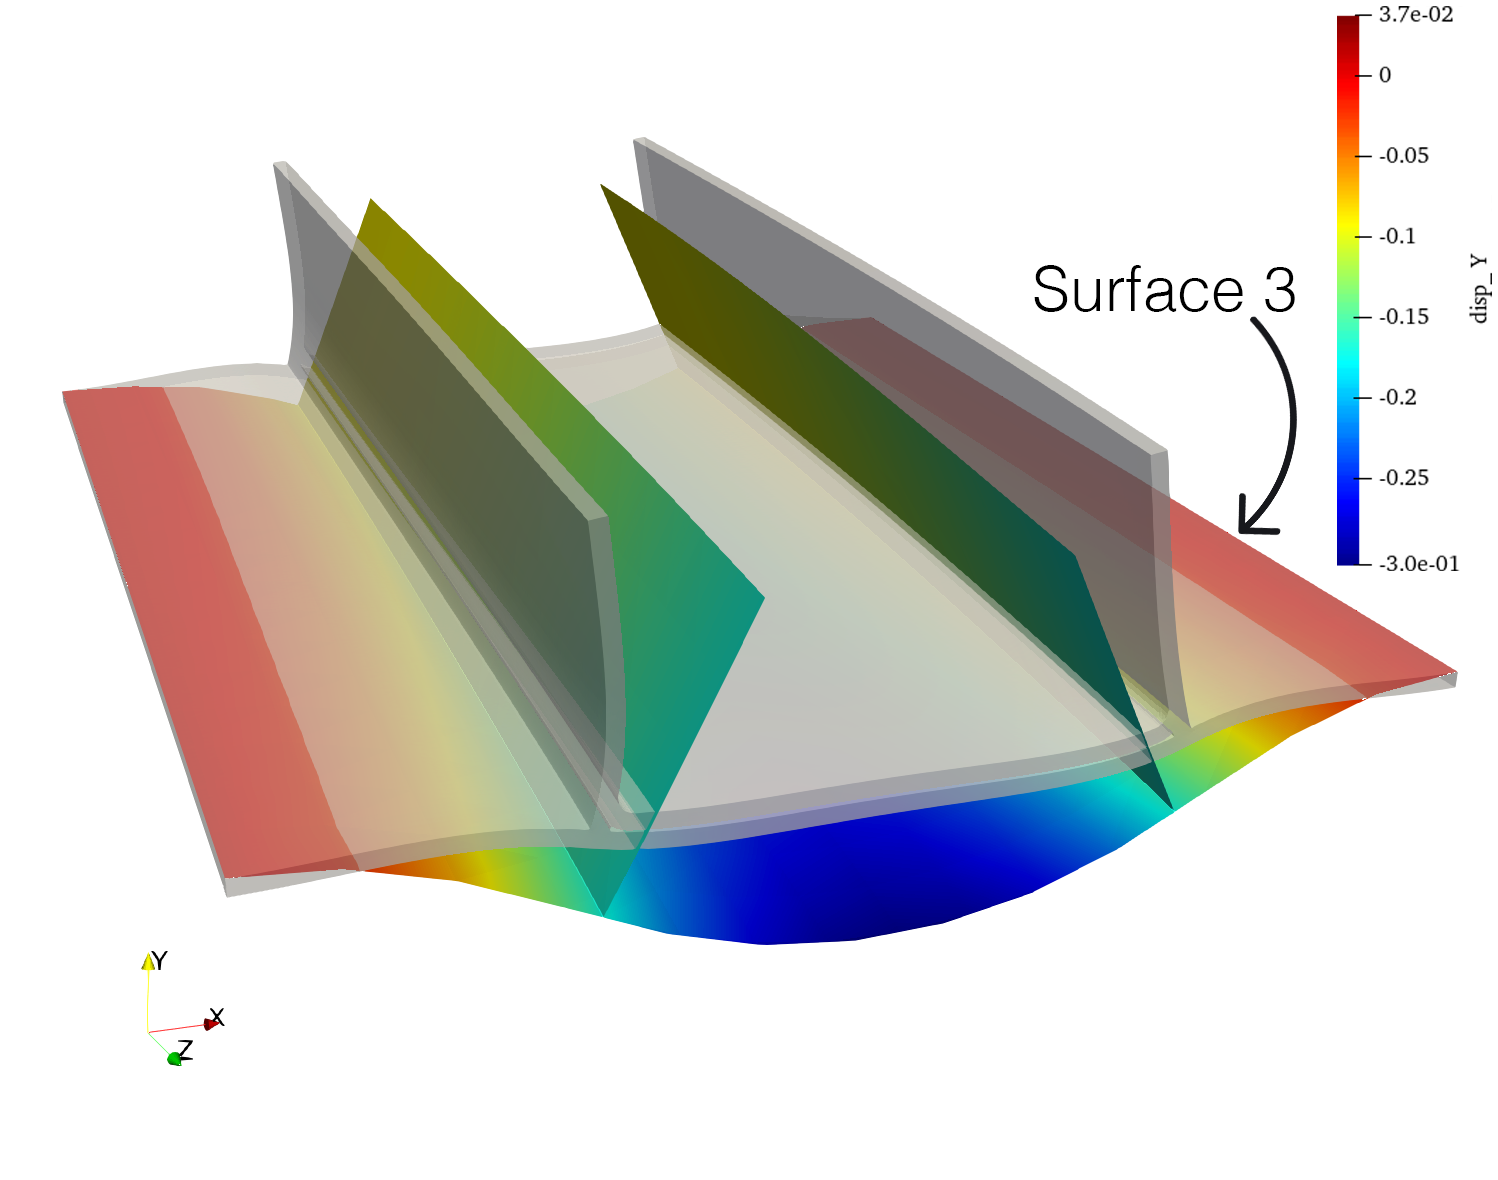
\includegraphics[width=0.65\textwidth,height=\textwidth,keepaspectratio]{2d_mesh_converge_coarse.png}
\caption{Comparison of the structural model and continuum model displacements for the x-displaced surface 3 BC. The mesh size is 12.7 mm. Displacements are magnified 1000x.
}
\label{fig:2d_mesh_converge_coarse}
\end{figure}

\begin{figure}[h!]
\centering
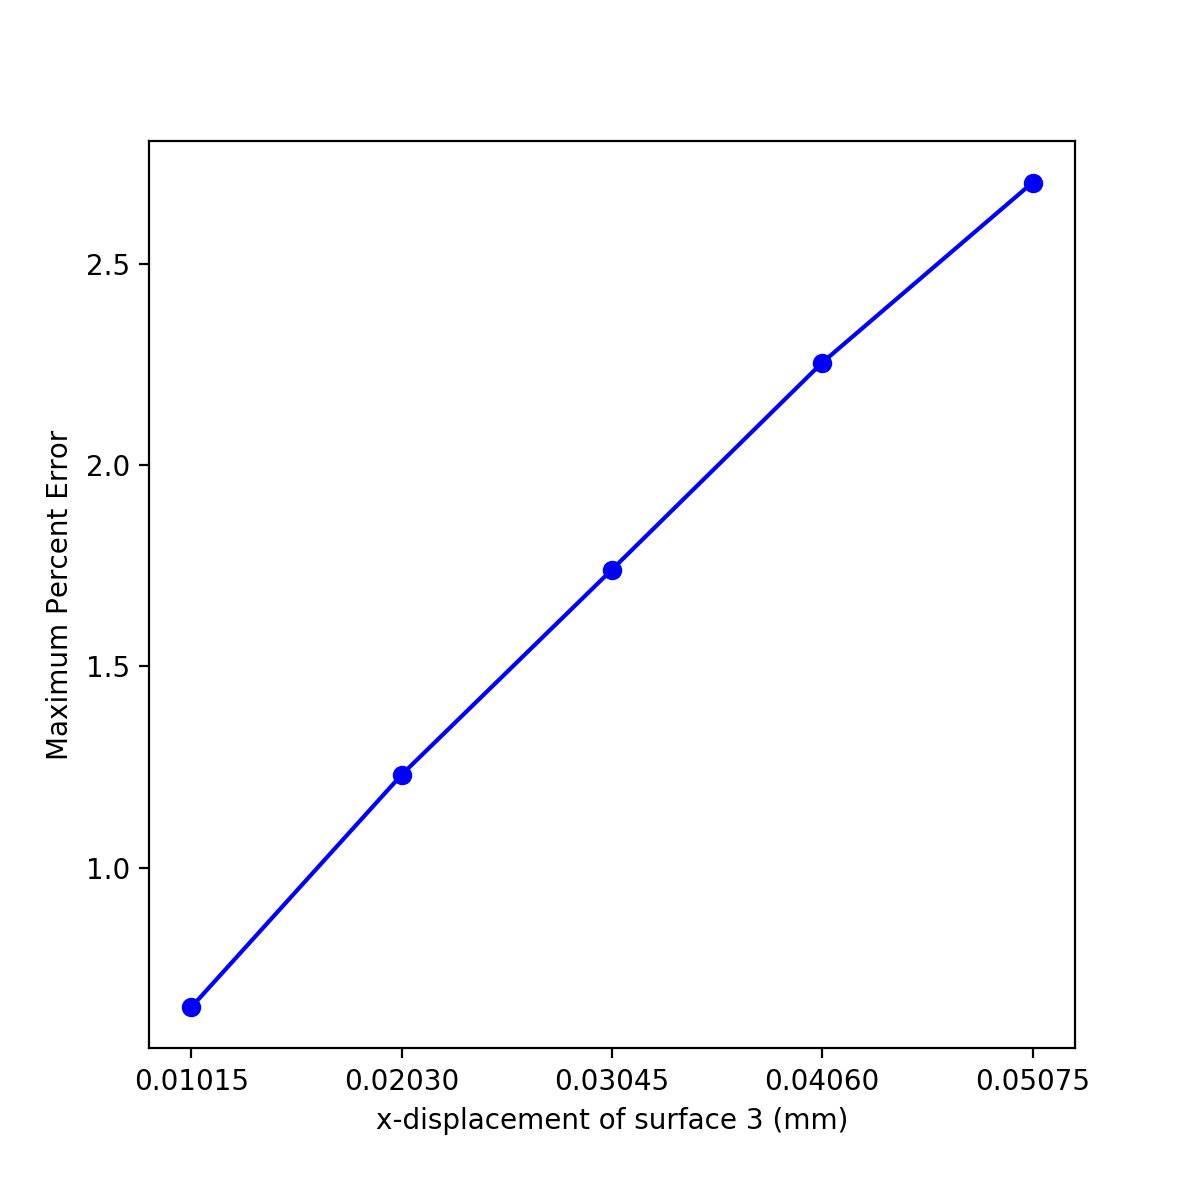
\includegraphics[width=0.65\textheight,height=300pt,keepaspectratio]{nl_sload_error.png}
\caption{The largest percent difference out of 609 points spaced equally across
the model plotted with respect to the applied displacement of surface 3.}
\label{fig:nl_sload_error}
\end{figure}

\begin{figure}[h!]
\centering
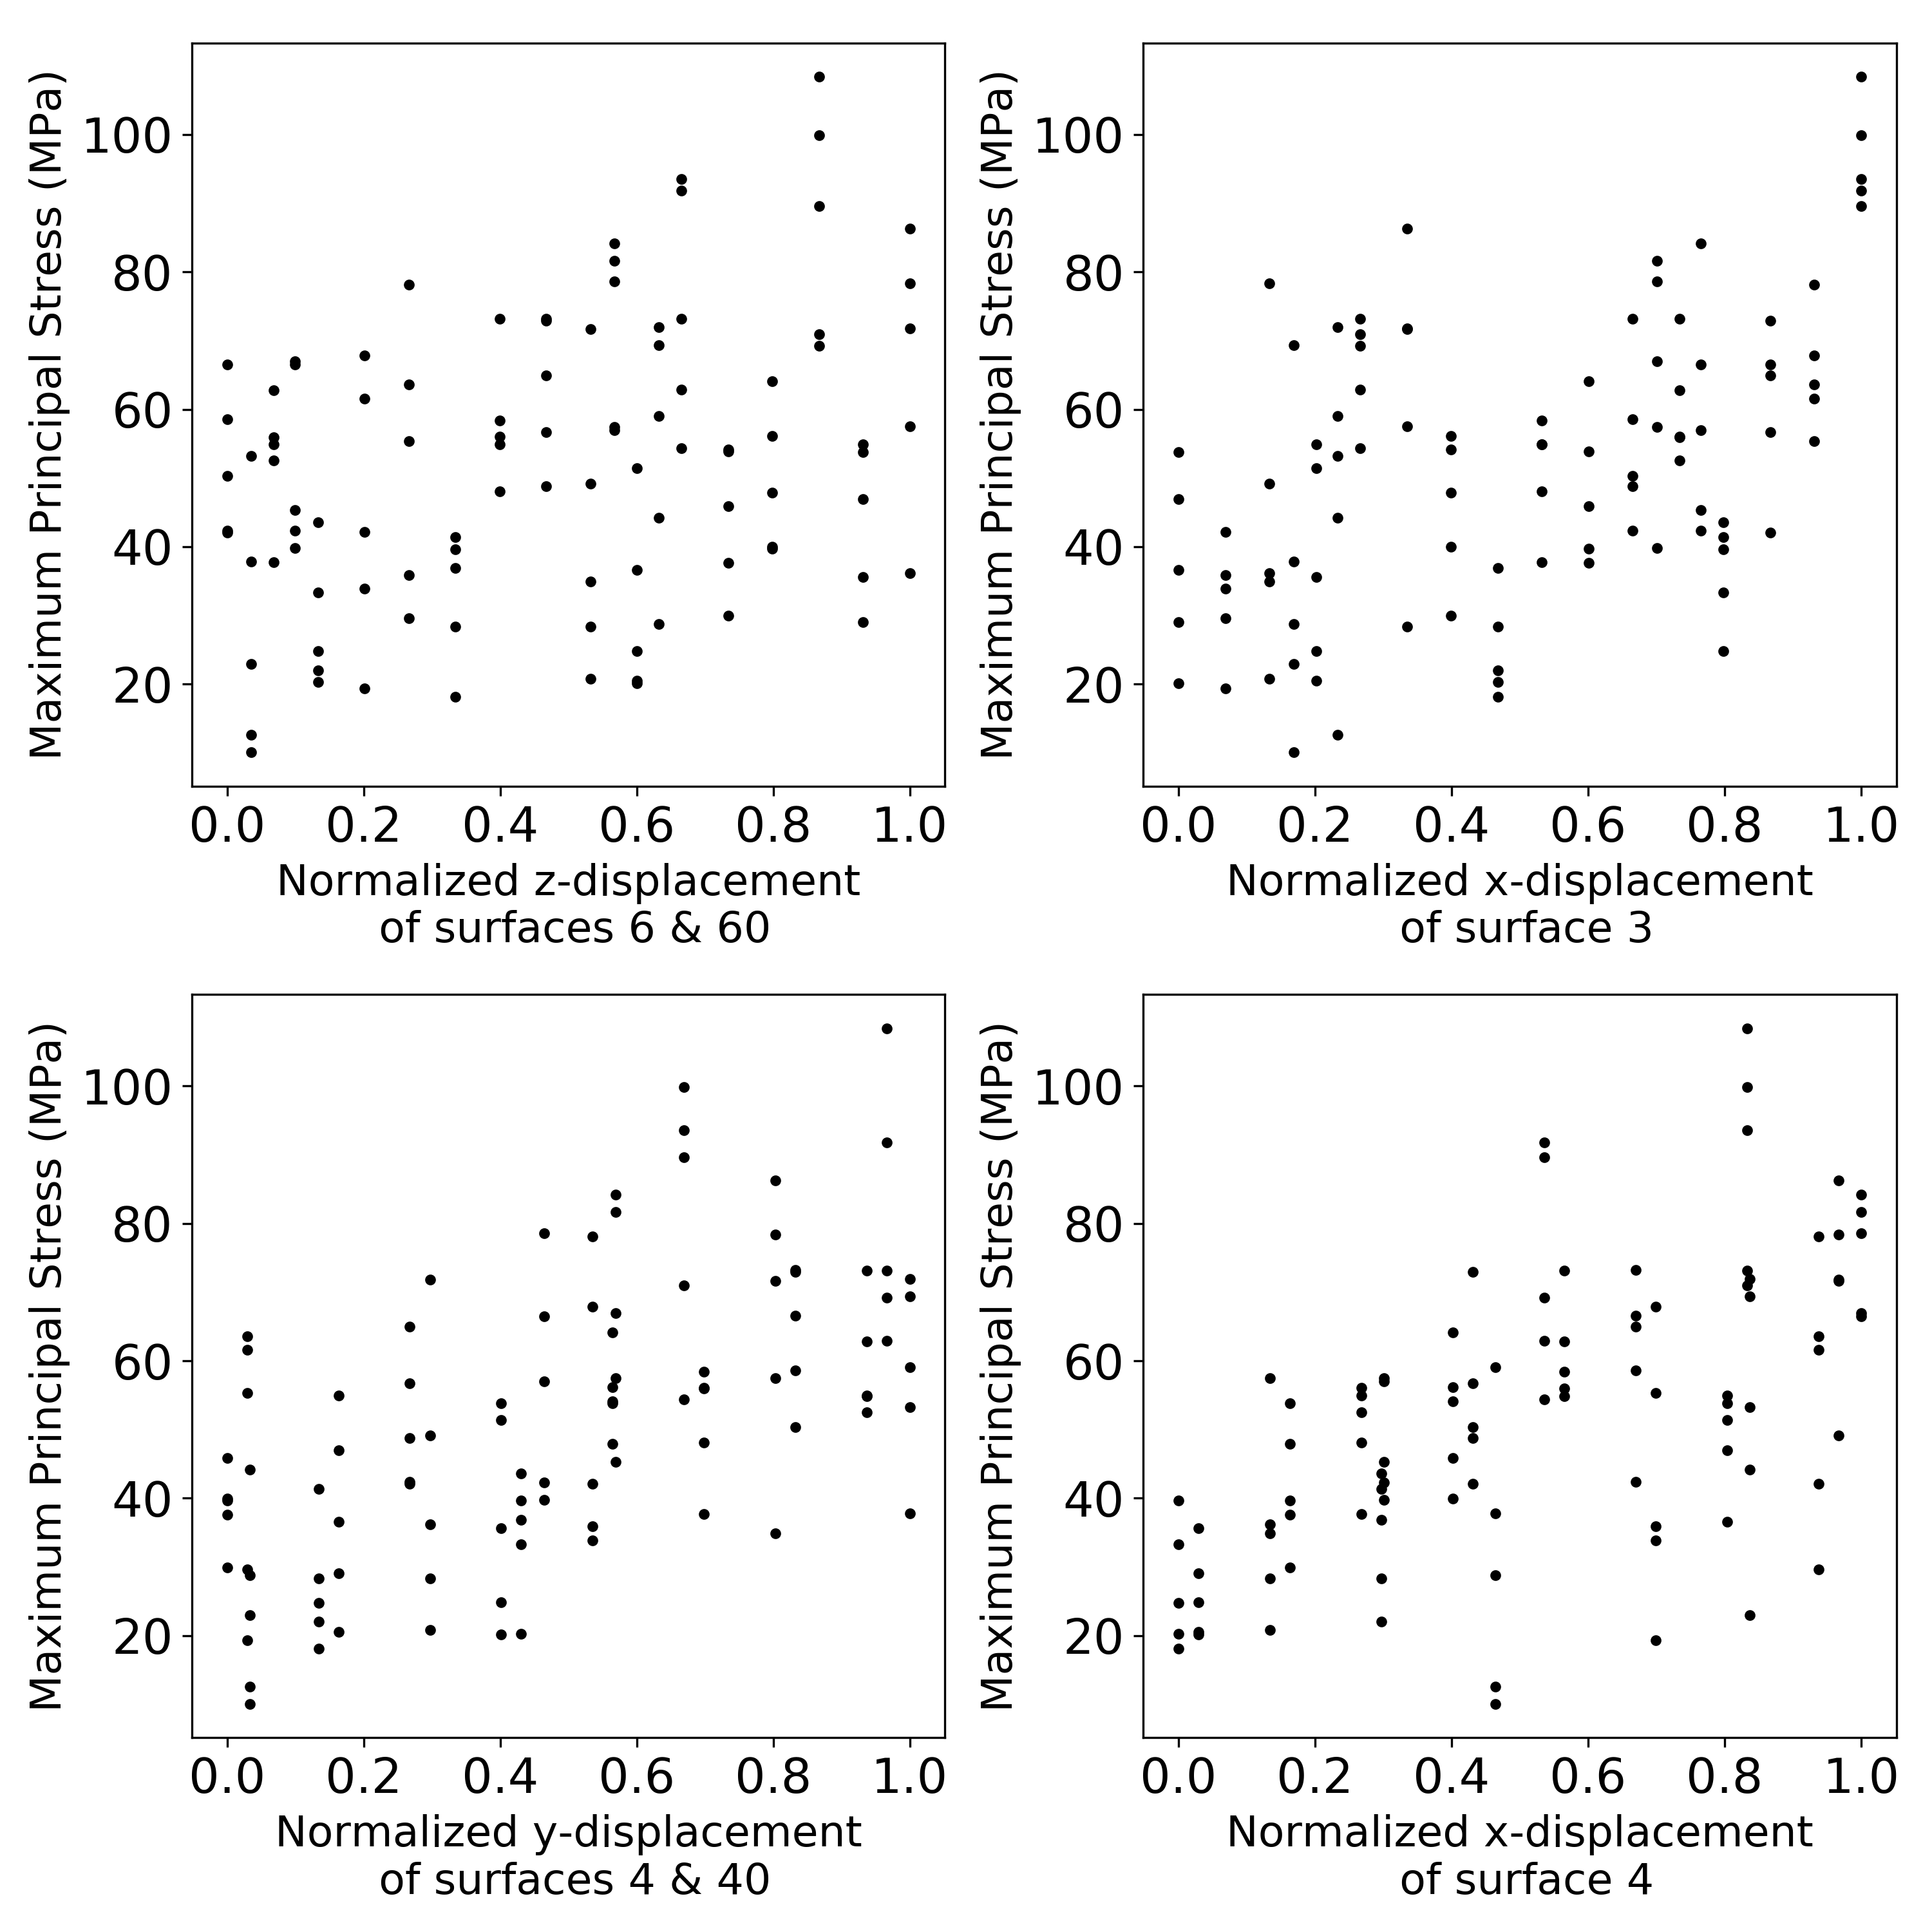
\includegraphics[width=0.6\textwidth,keepaspectratio]{MPS_vs_rstl.png}
\caption{Effects of each boundary condition on the maximum principal stress at a
point in the weld surface center. The point from which the maximum
principal stress is calculated is illustrated in Figure
\ref{fig:local_mps_point}. Displacements are normalized by their maximum applied
displacement BC.
}
\label{fig:mps_vs_rstl}
\end{figure}

\begin{figure}[h!]
\centering
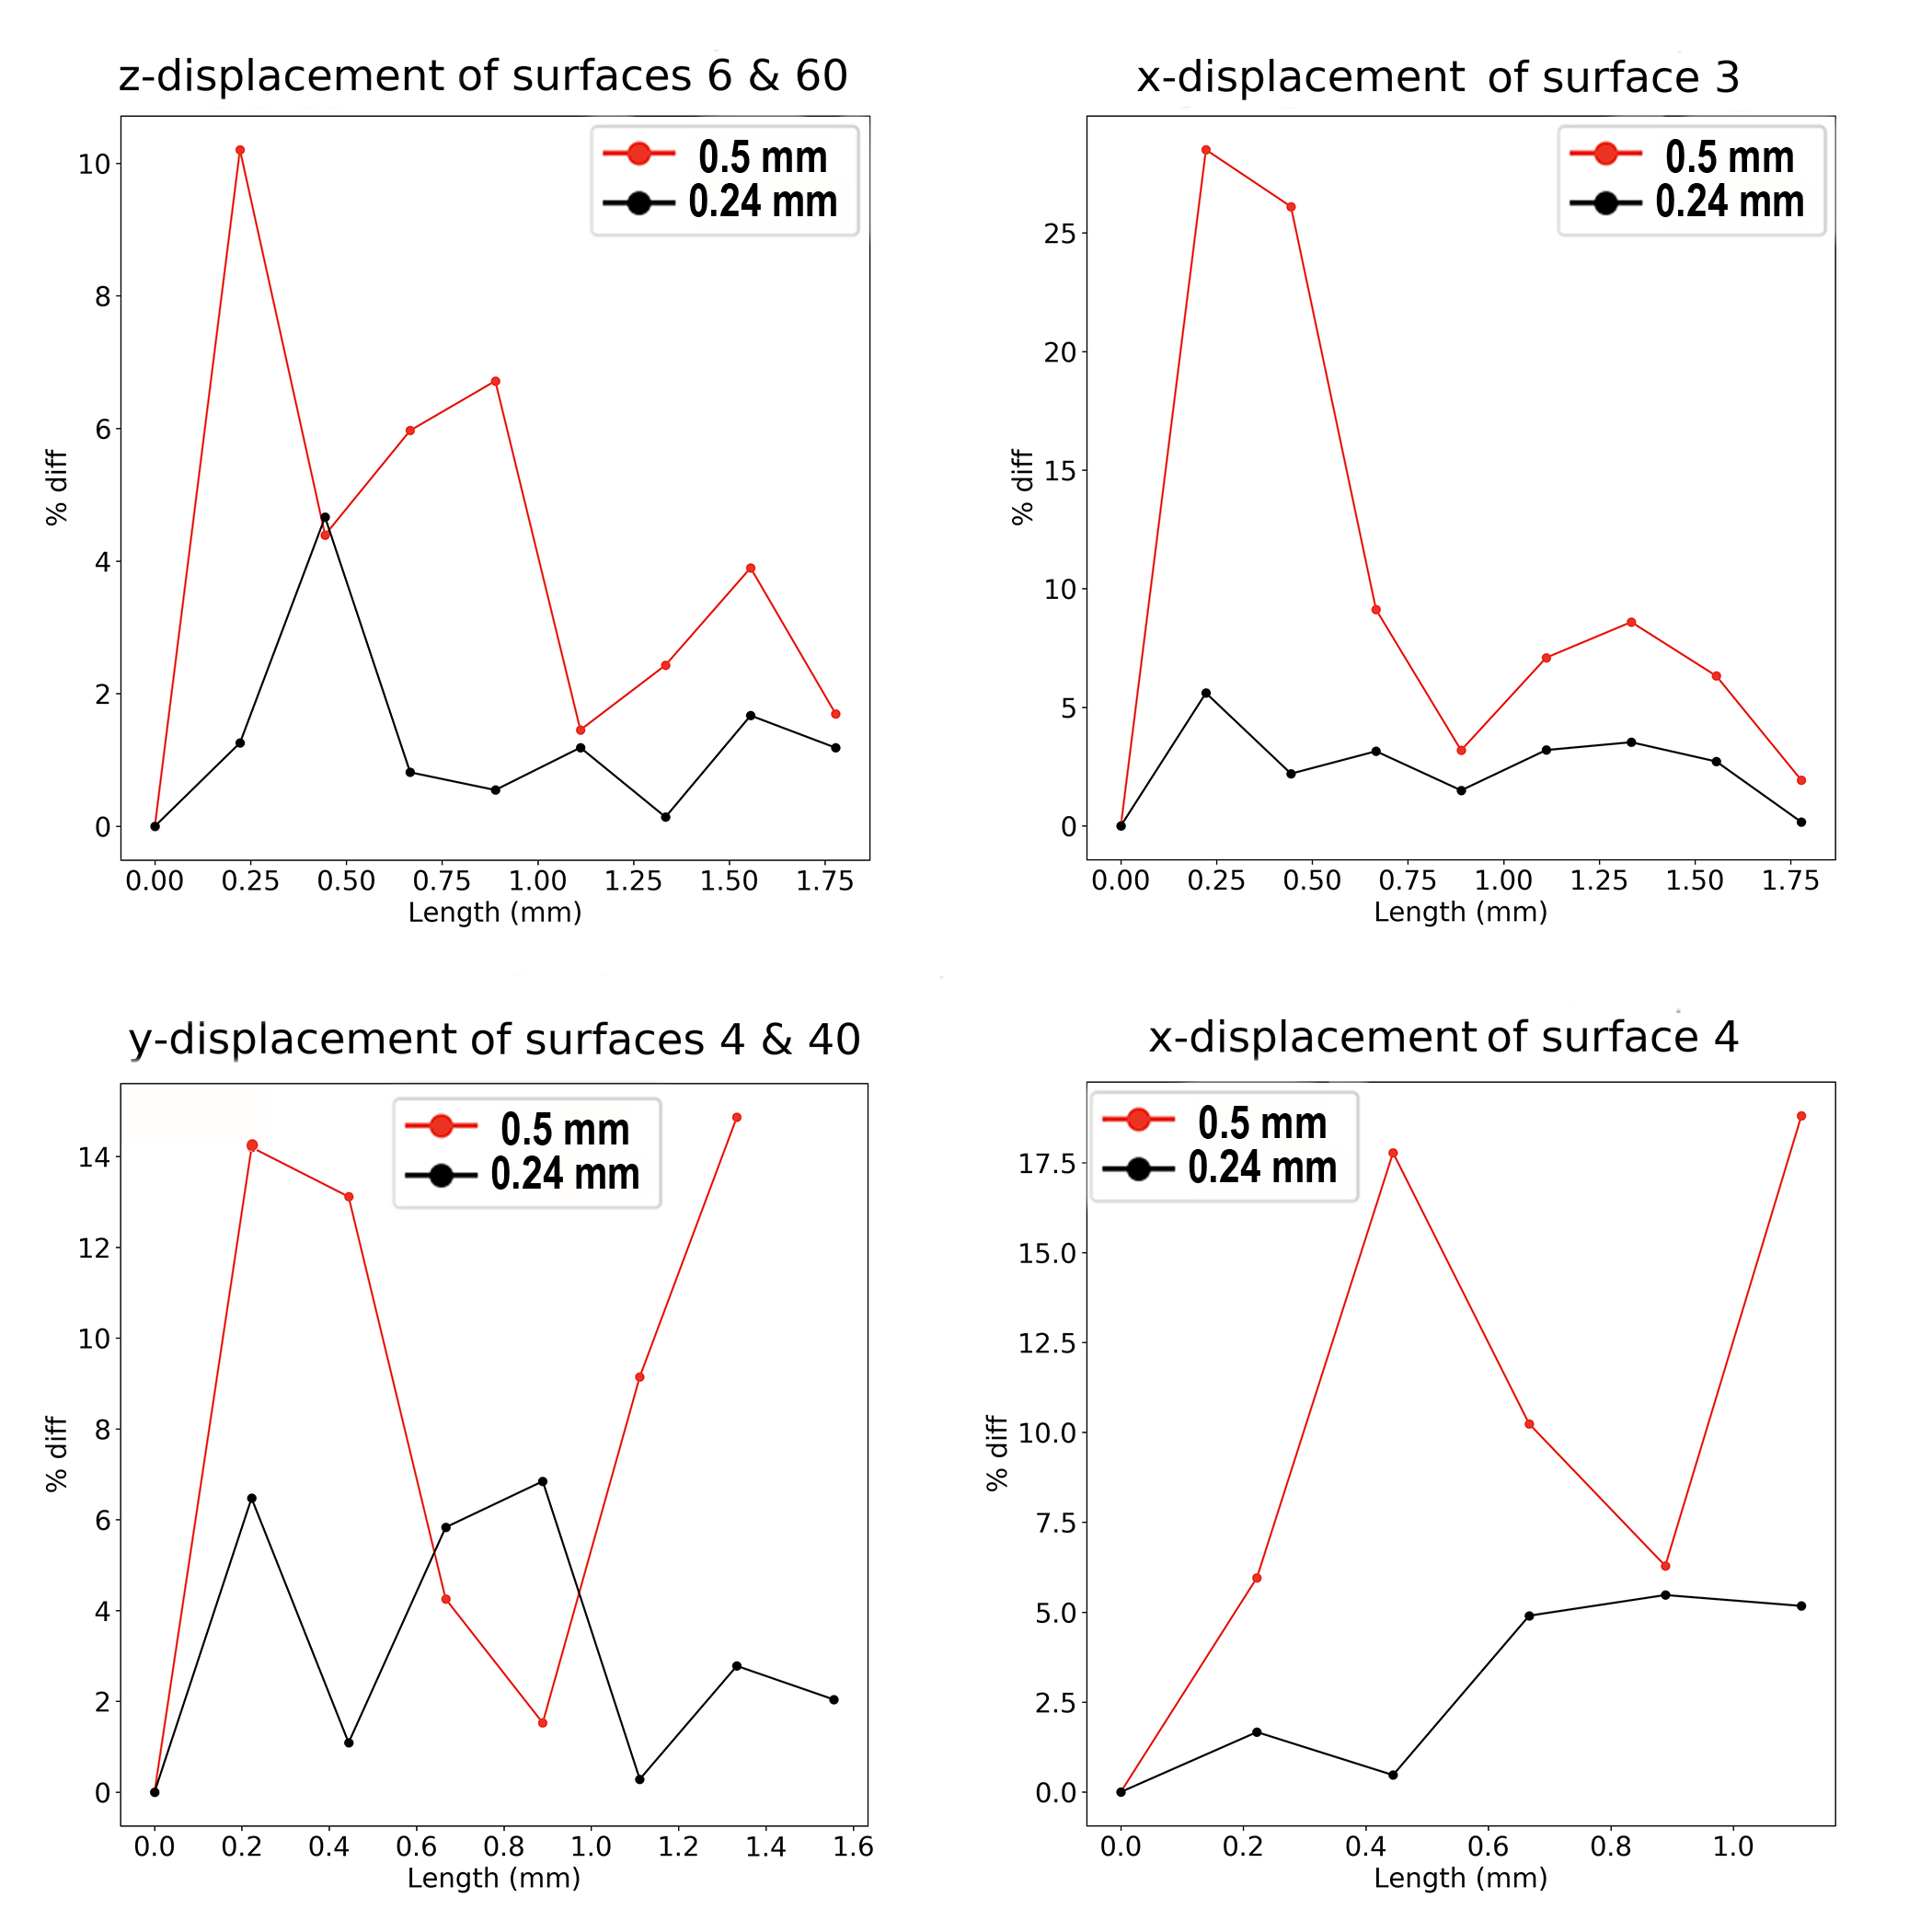
\includegraphics[width=\textwidth,height=\textheight,keepaspectratio]{crack_convergence.png}
\caption{Convergence of crack growth step size for each of the four different
displacement boundary conditions. The percent difference is calculated with respect
to a 0.15 mm crack growth step size.
}
\label{fig:crack_convergence}
\end{figure}

\begin{figure}[h!]
  \begin{subfigure}[b]{0.5\textwidth}
    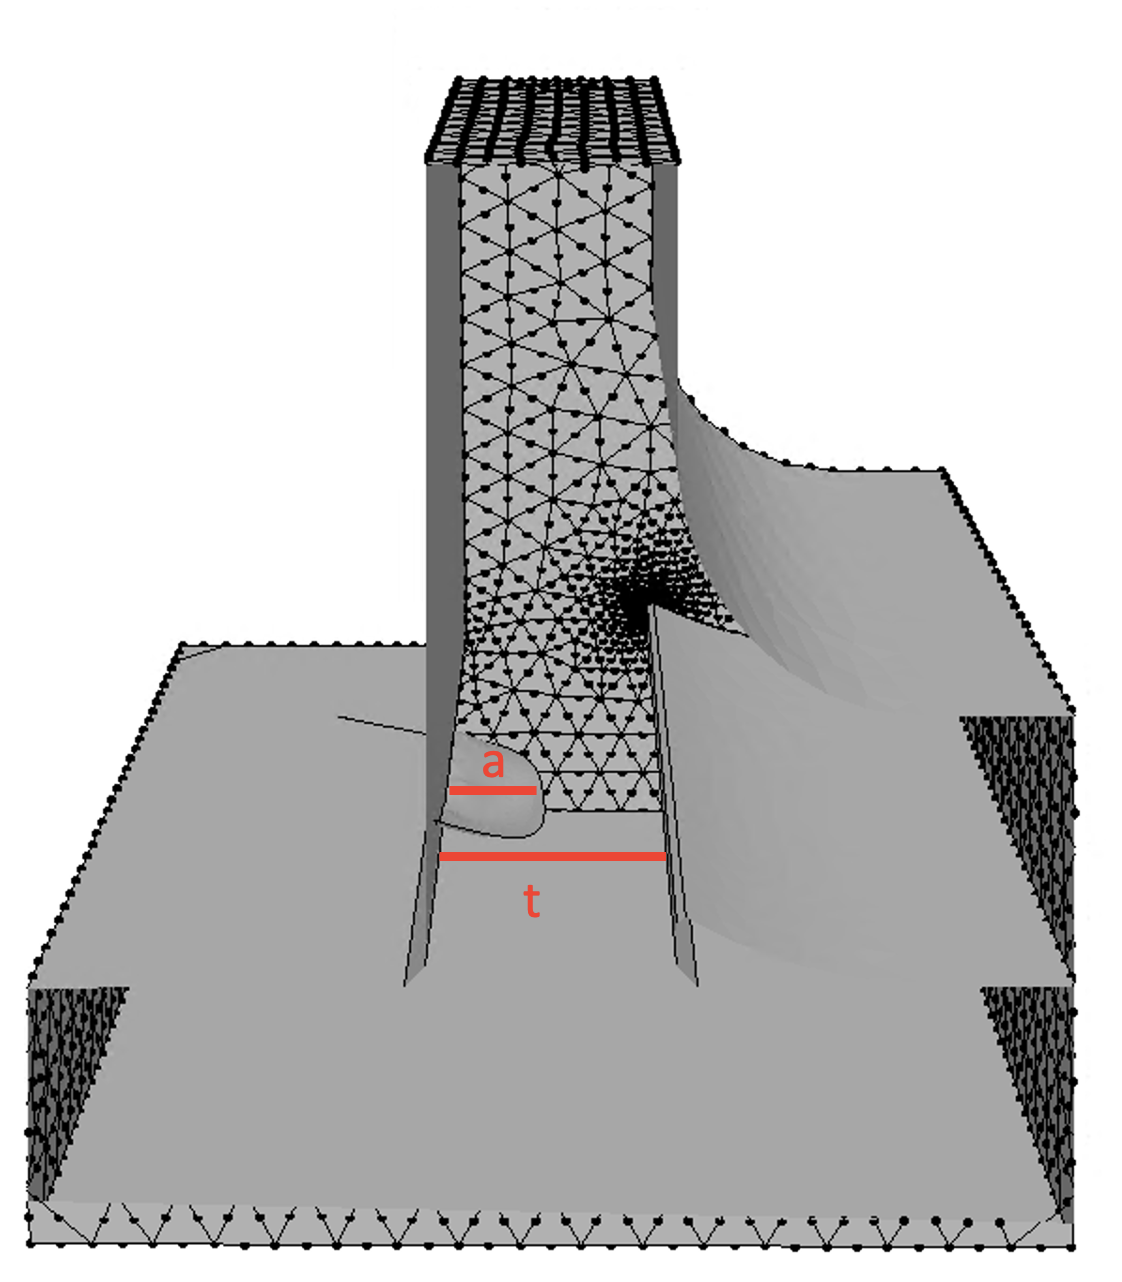
\includegraphics[width=\textwidth]{horizontal_growth.png}
    \caption{Horizontal growth path}
    \label{fig:horizontal_growth}
  \end{subfigure}
  \hfill
  \begin{subfigure}[b]{0.5\textwidth}
    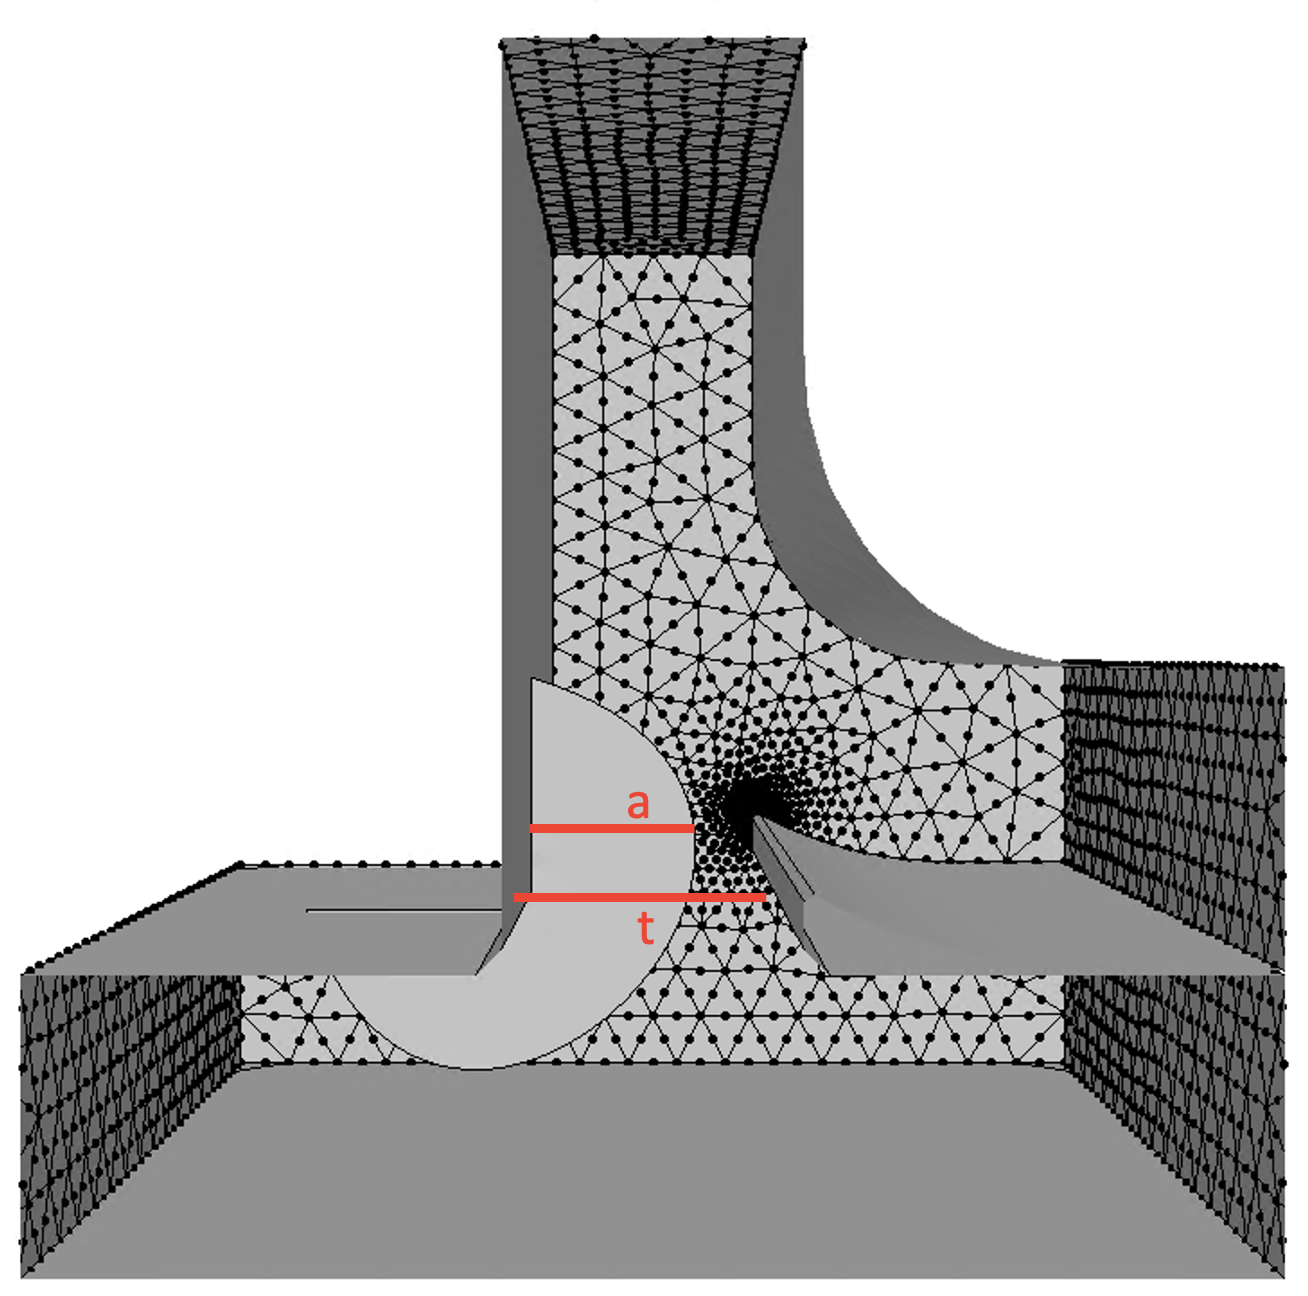
\includegraphics[width=\textwidth]{horizontal_growth2.png}
    \caption{Horizontal growth path}
    \label{fig:horizontal_growth2}
  \end{subfigure}
  \hfill
  \begin{subfigure}[b]{0.5\textwidth}
    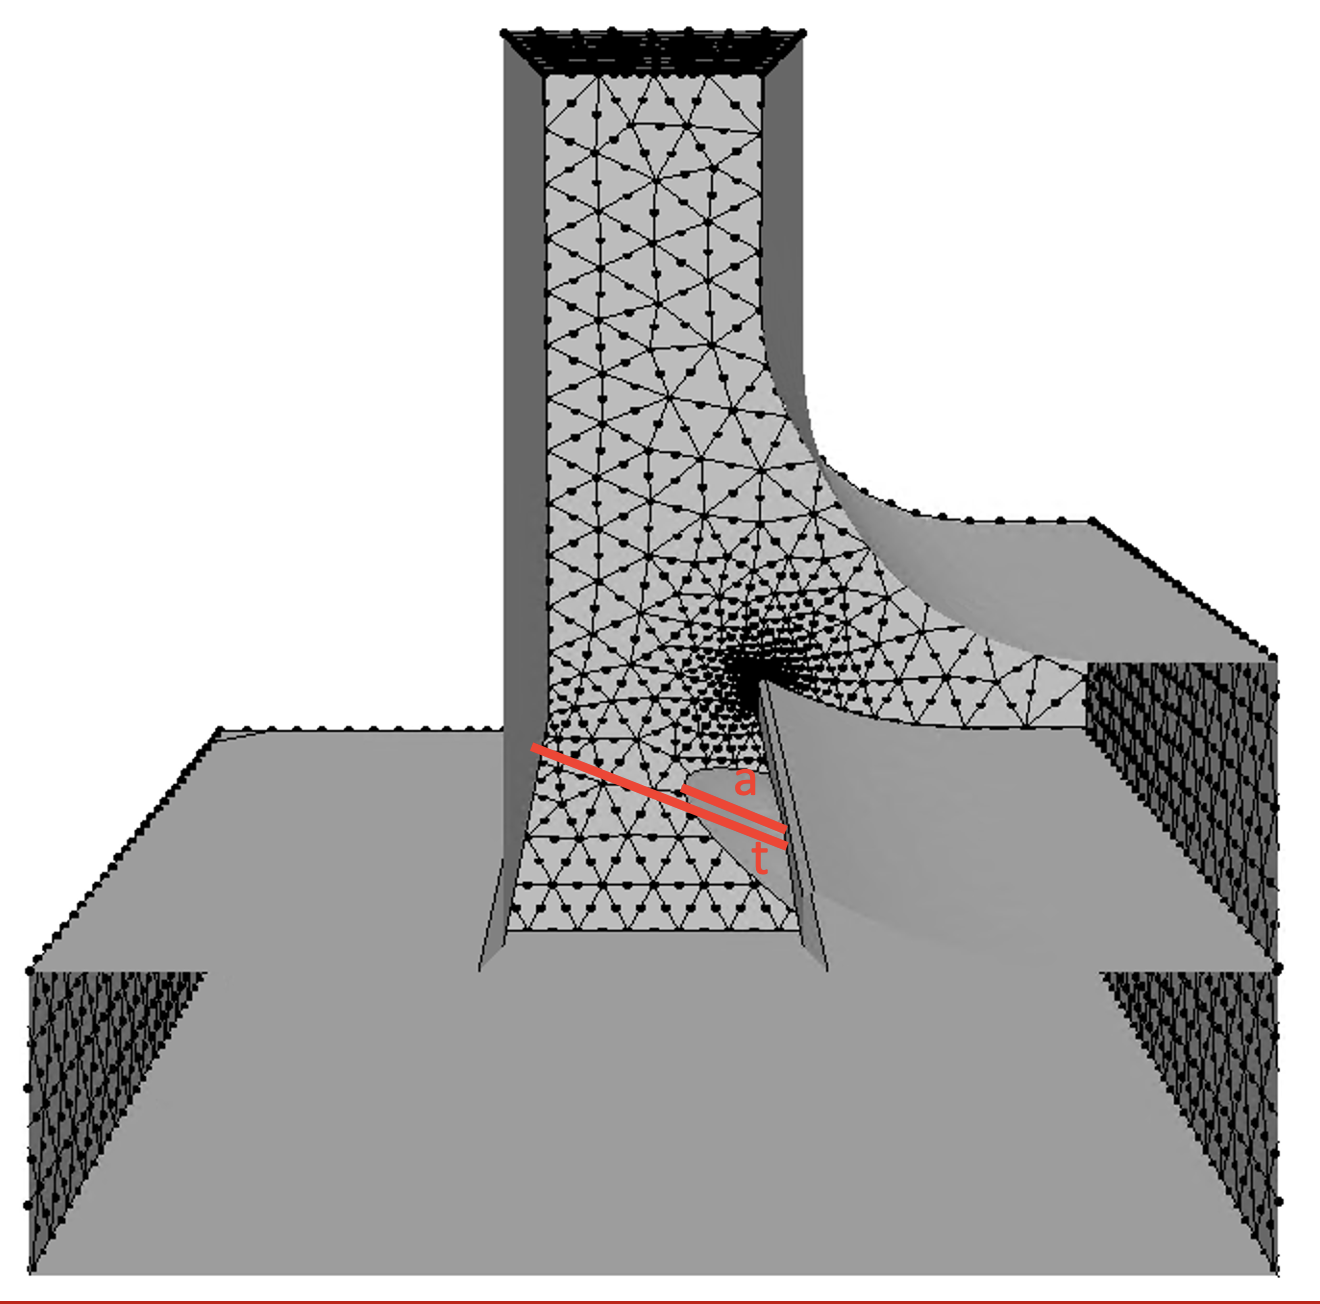
\includegraphics[width=\textwidth]{upward_growth.png}
    \caption{Horizontal upward growth path}
    \label{fig:upward_growth}
  \end{subfigure}
  \hfill
  \begin{subfigure}[b]{0.5\textwidth}
    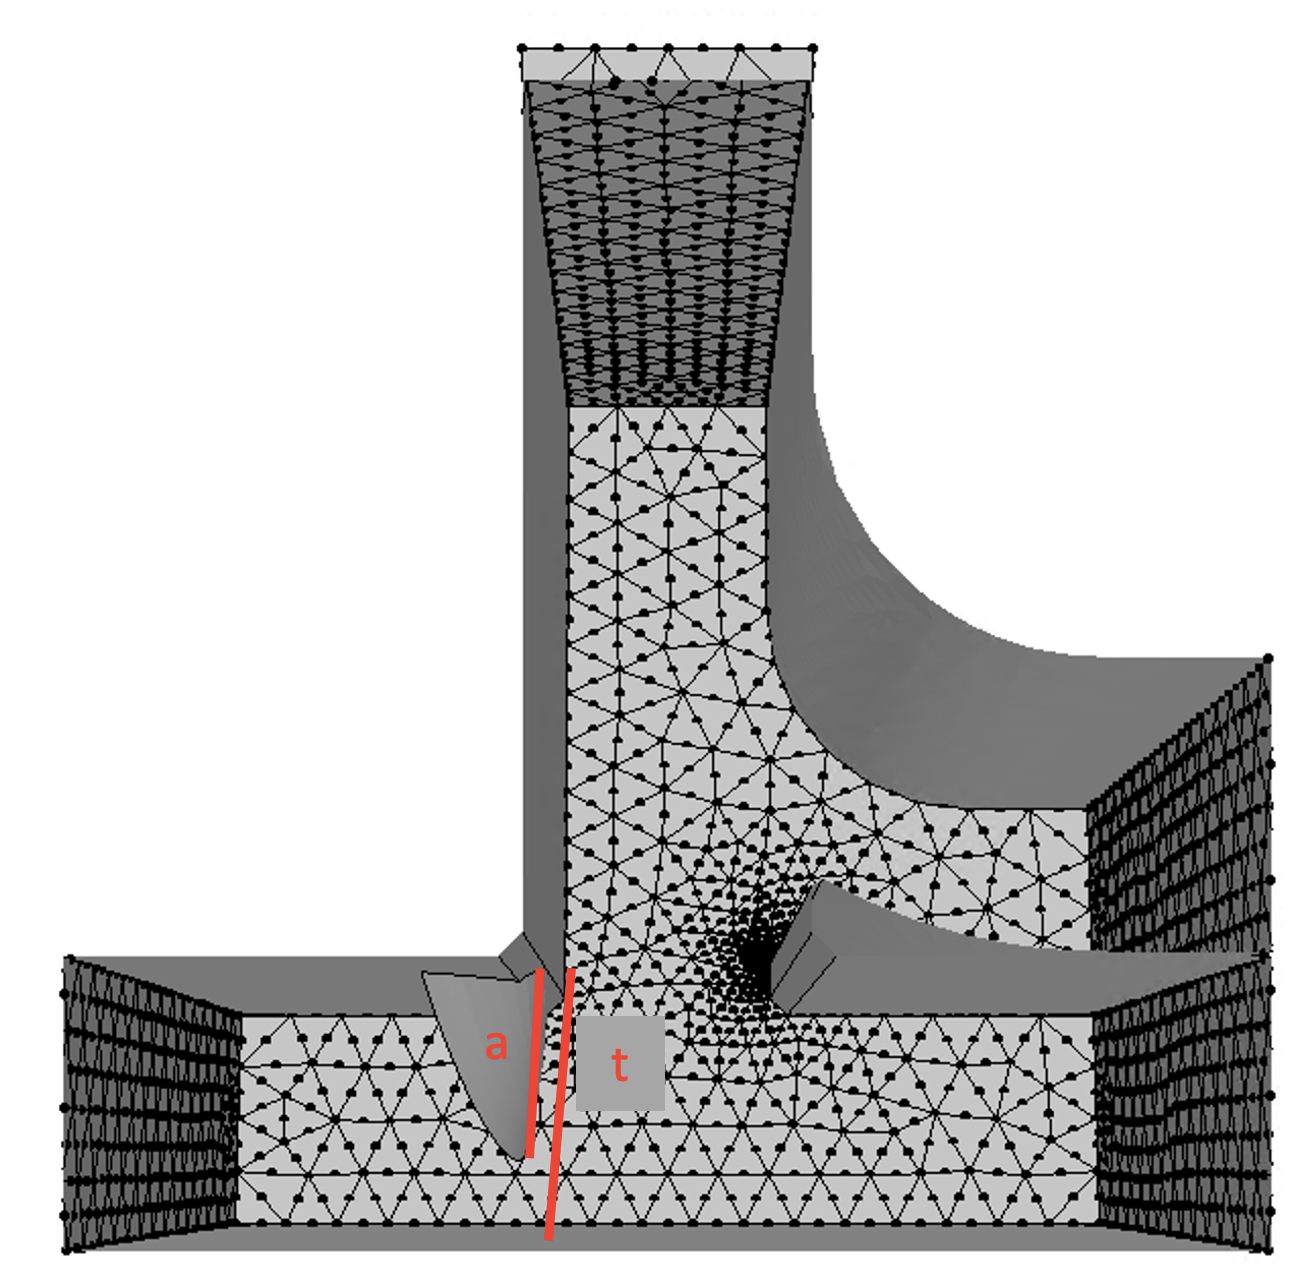
\includegraphics[width=\textwidth]{downward_growth.png}
    \caption{Downward growth}
    \label{fig:downward_growth}
  \end{subfigure}
  \caption{Four examples illustrating the variety of different growth paths the
cracks followed. Each figure shows how both the crack depth $a$ and the thickness
$t$ were defined in the different cases.}
  \label{fig:crack_paths}
\end{figure}

\begin{figure}[h!]
\centering
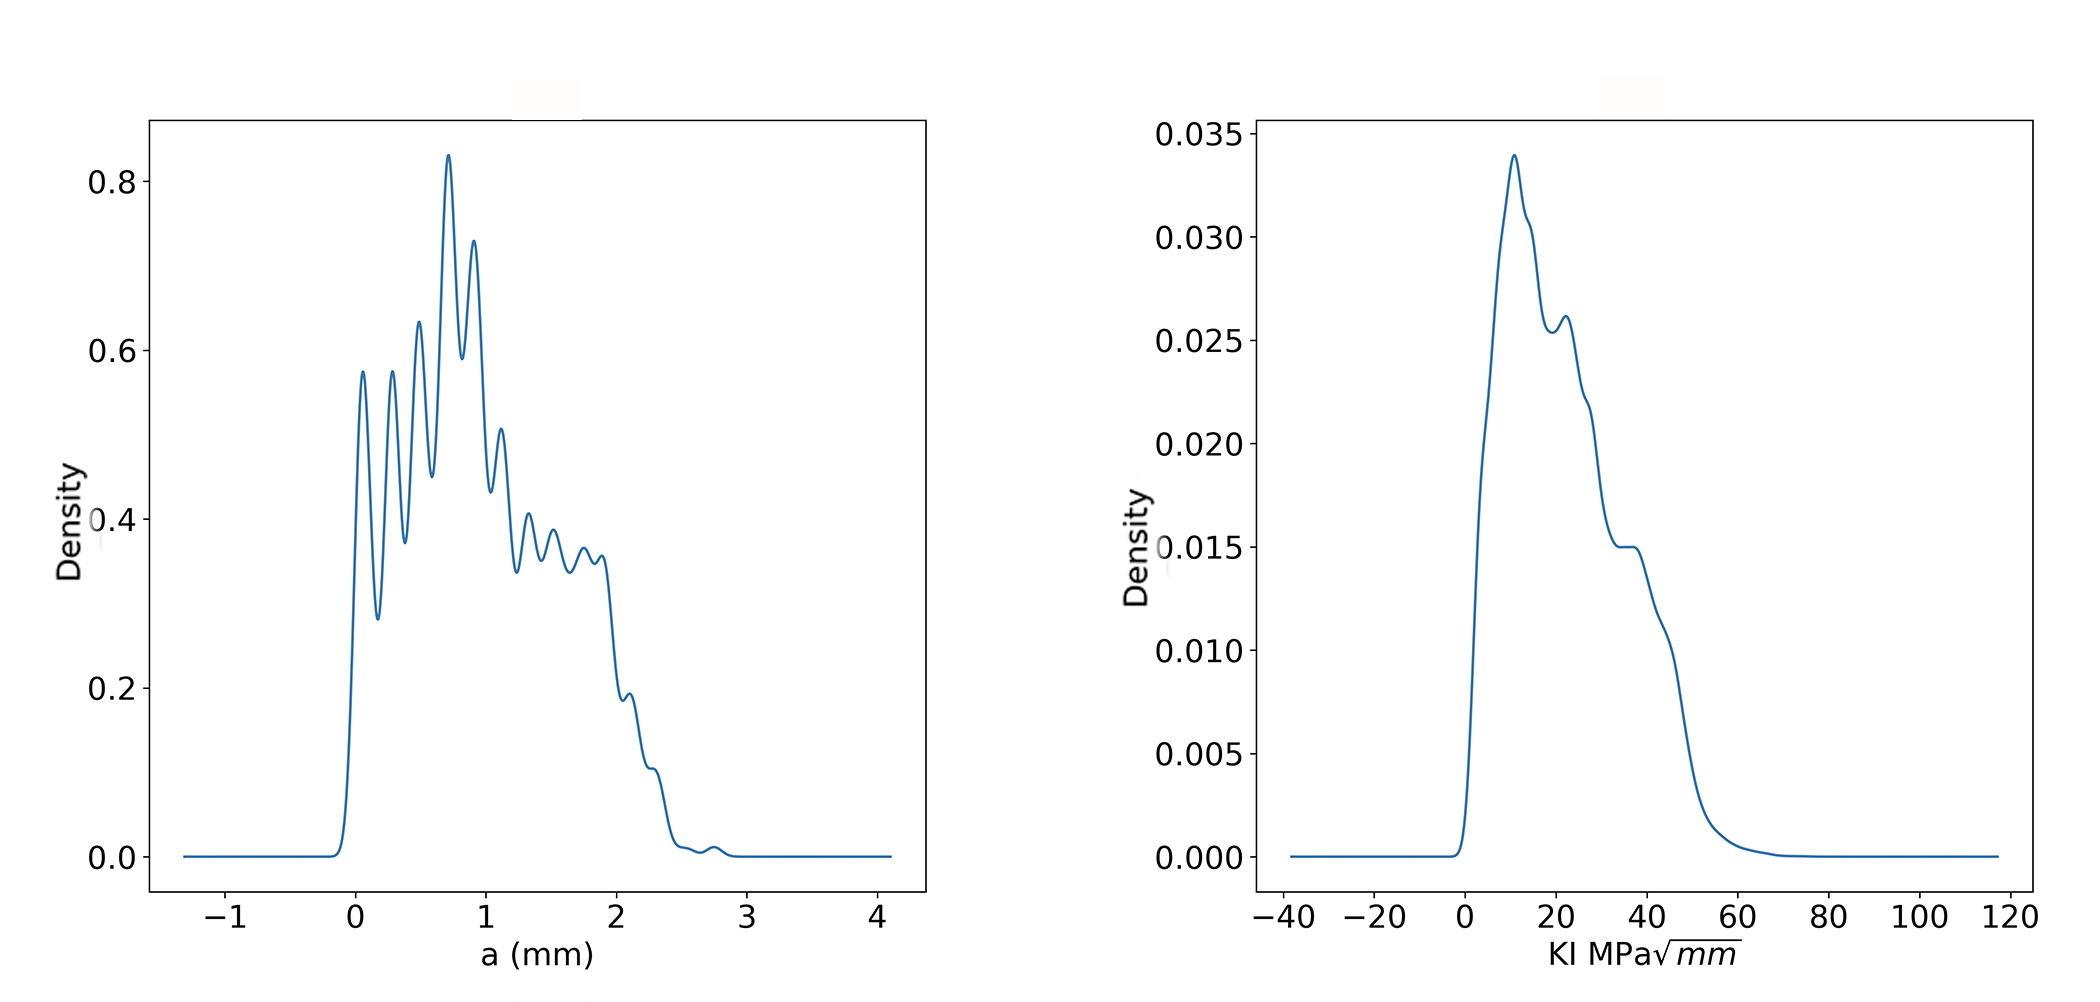
\includegraphics[width=\textwidth,height=300pt,keepaspectratio]{aKI_pde.png}
\caption{Density curves of two of the variables calculated as a result of
computational fracture analysis. Crack depth, a, and $K_I$.
}
\label{fig:aKI_pde}
\end{figure}

\begin{figure}[h!]
\centering
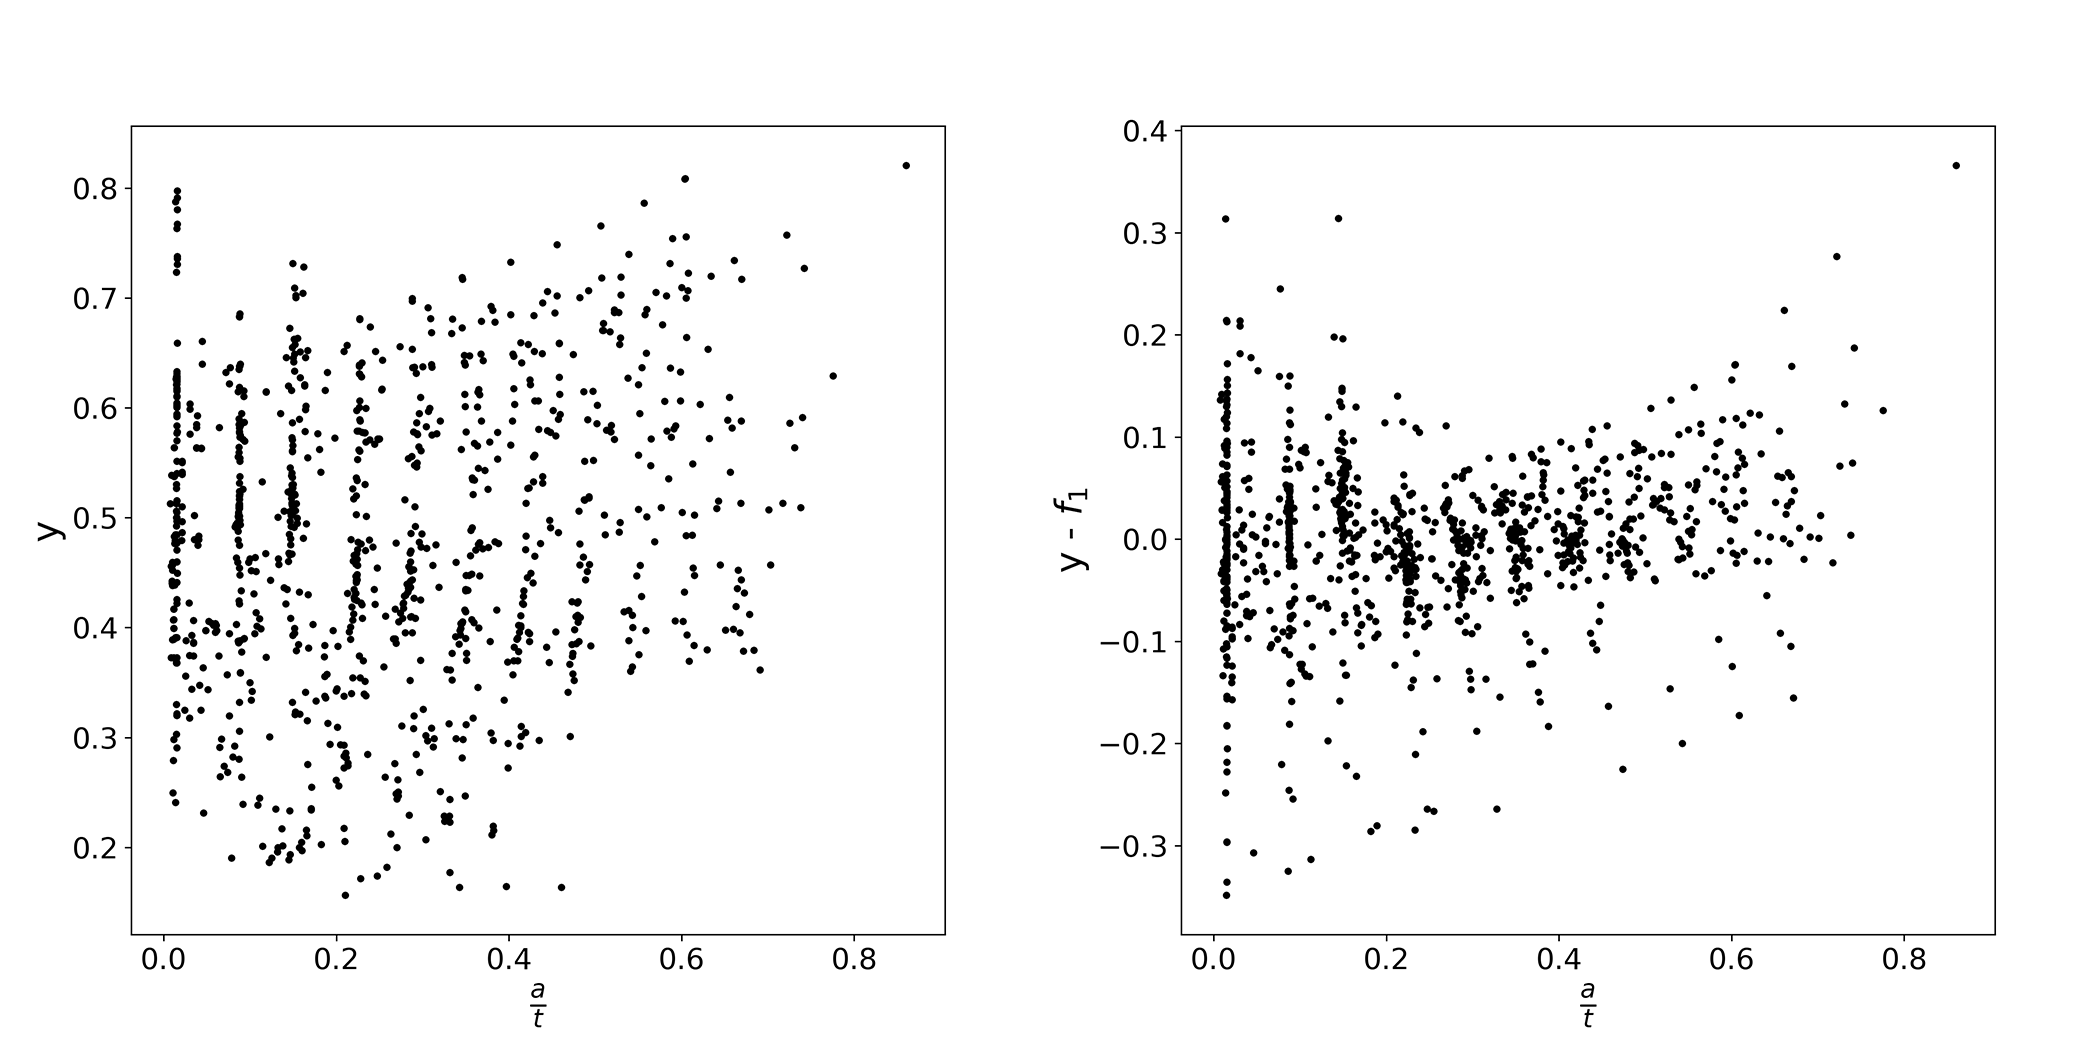
\includegraphics[width=\textwidth,height=300pt,keepaspectratio]{f_fsubm1.png}

\caption{Plots for the ground truth with respect to $\frac{a}{t}$ and the ground
truth subtracted by the first model with respect to $\frac{a}{t}$. Showing high
amounts of scatter in the ground truth.  }

\label{fig:f_fsubm1}
\end{figure}

\begin{figure}[h!]
\centering
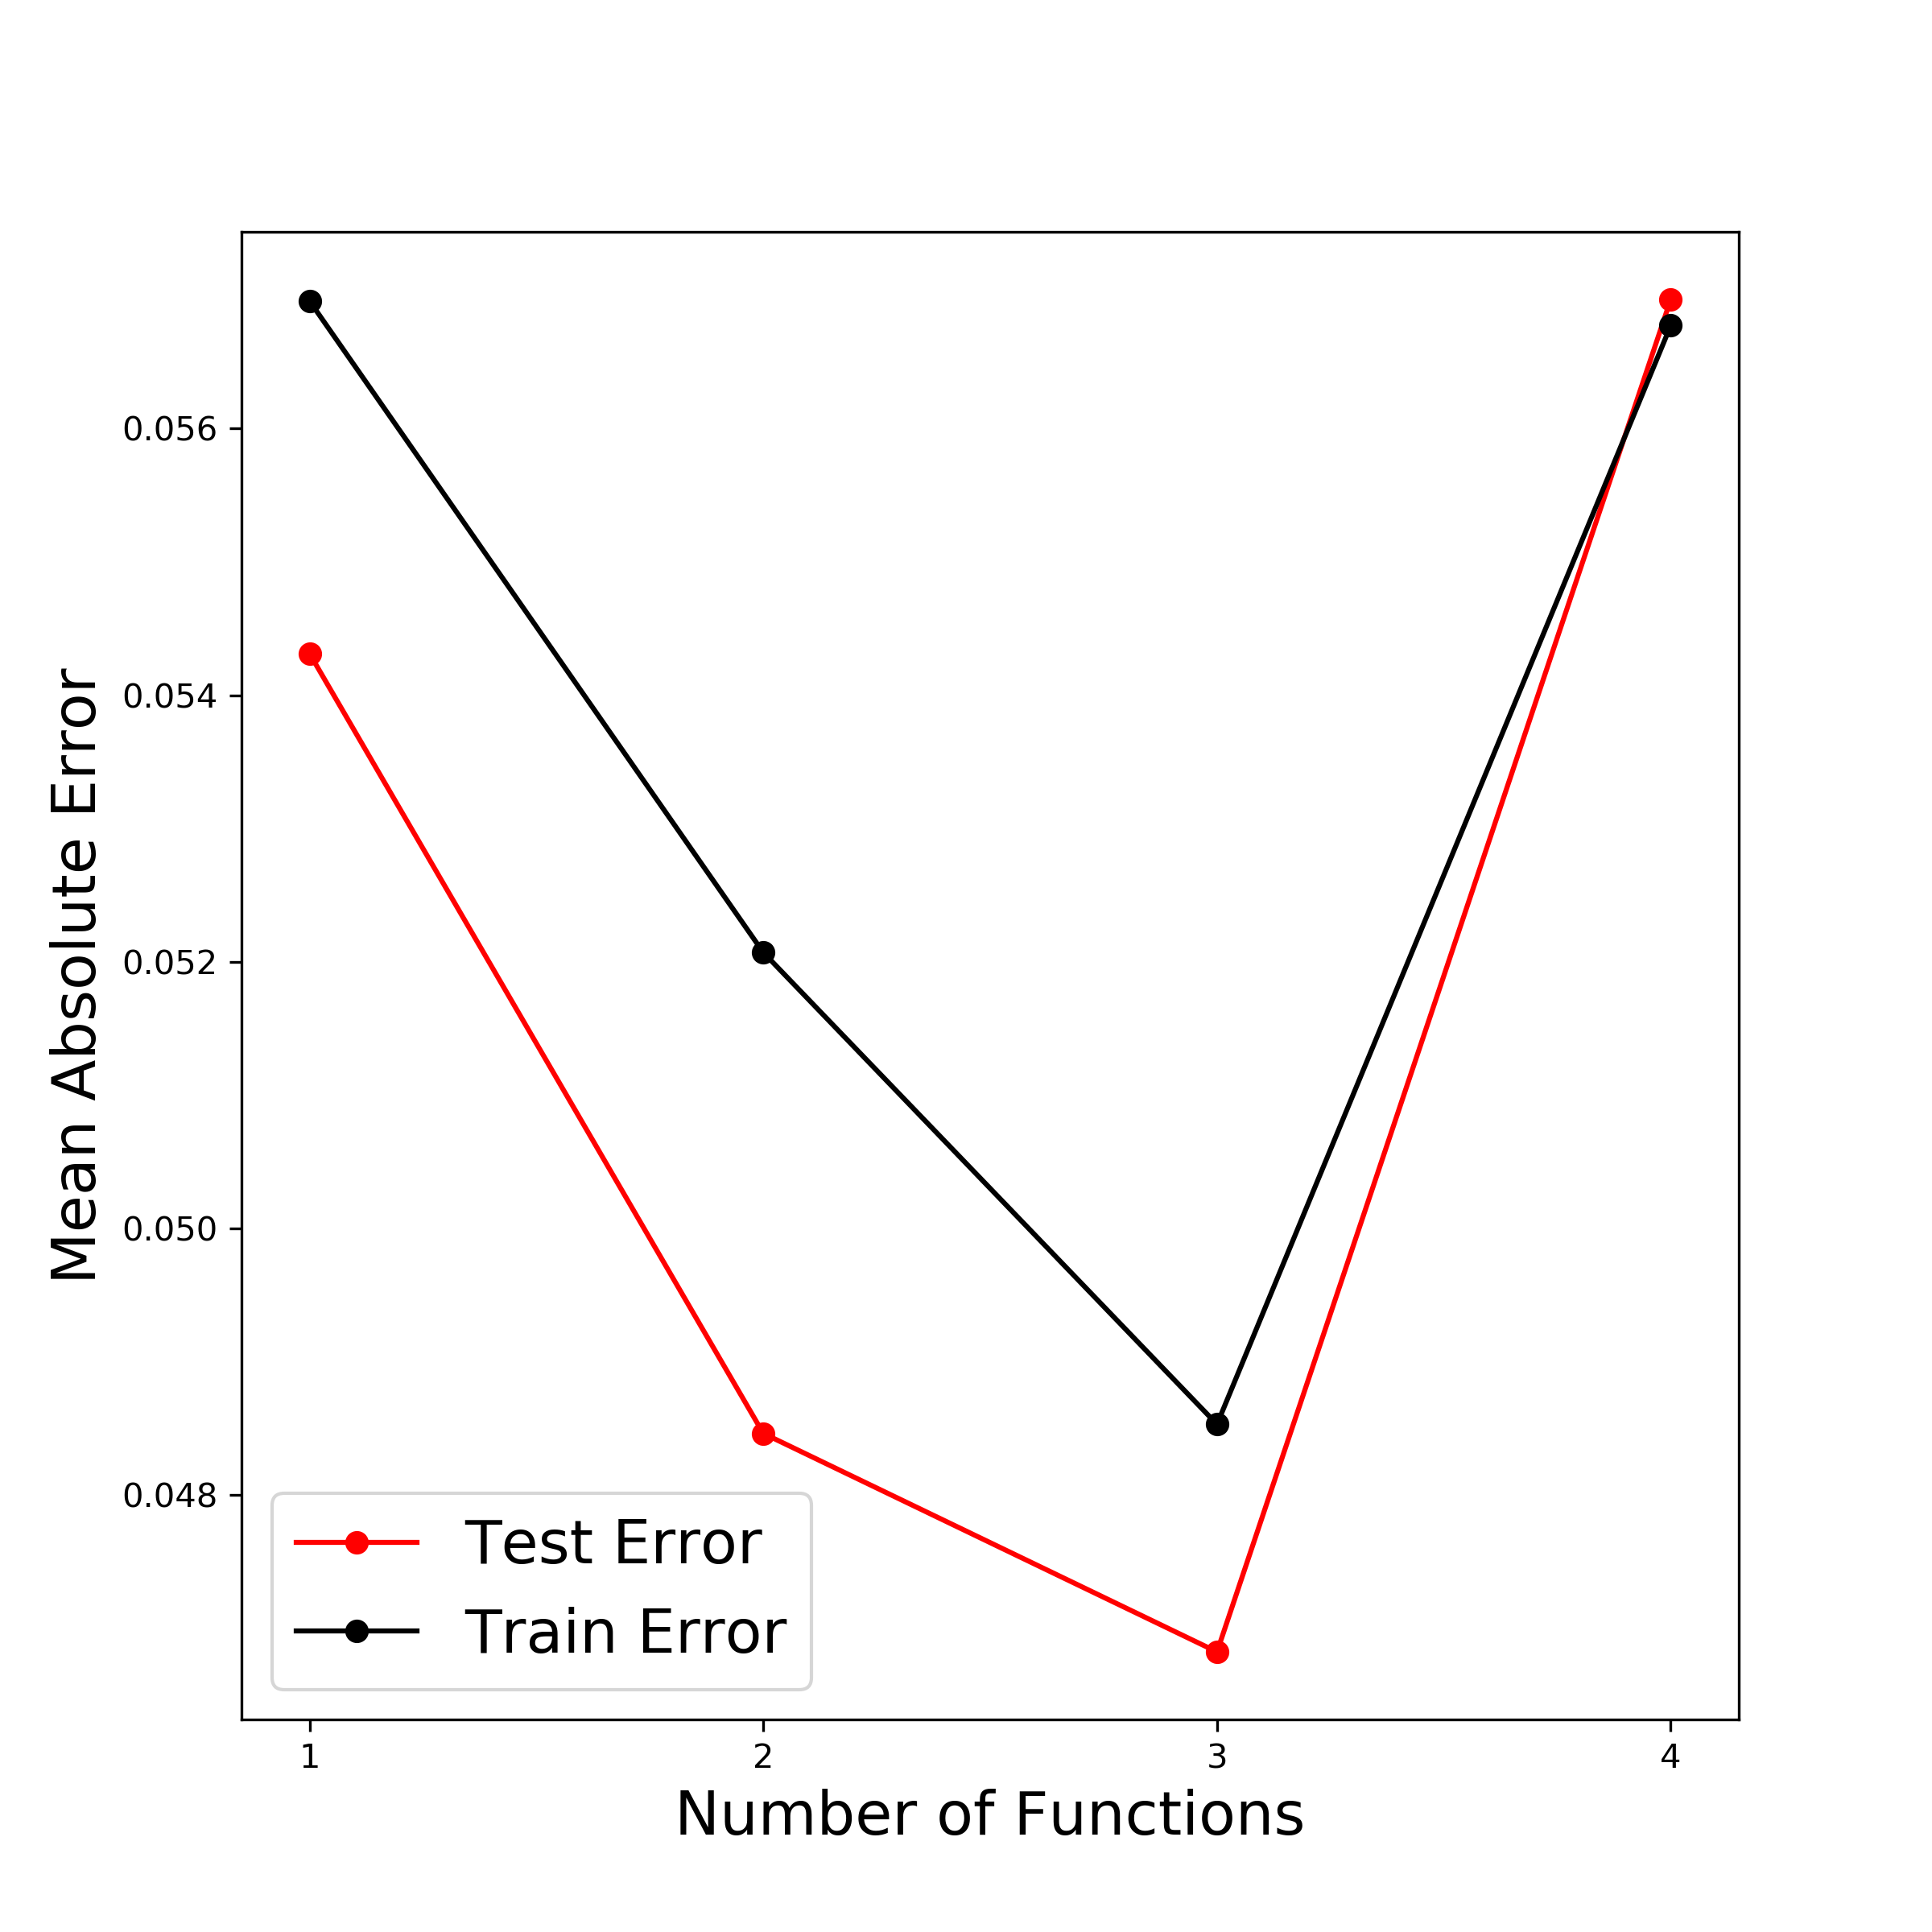
\includegraphics[width=\textwidth,height=300pt,keepaspectratio]{models_performance.png}

\caption{Mean absolute error of the training data and the test data with the
addition of more models.}
\label{fig:models_performance}
\end{figure}

\begin{figure}[h!]
  \begin{subfigure}[b]{0.5\textwidth}
    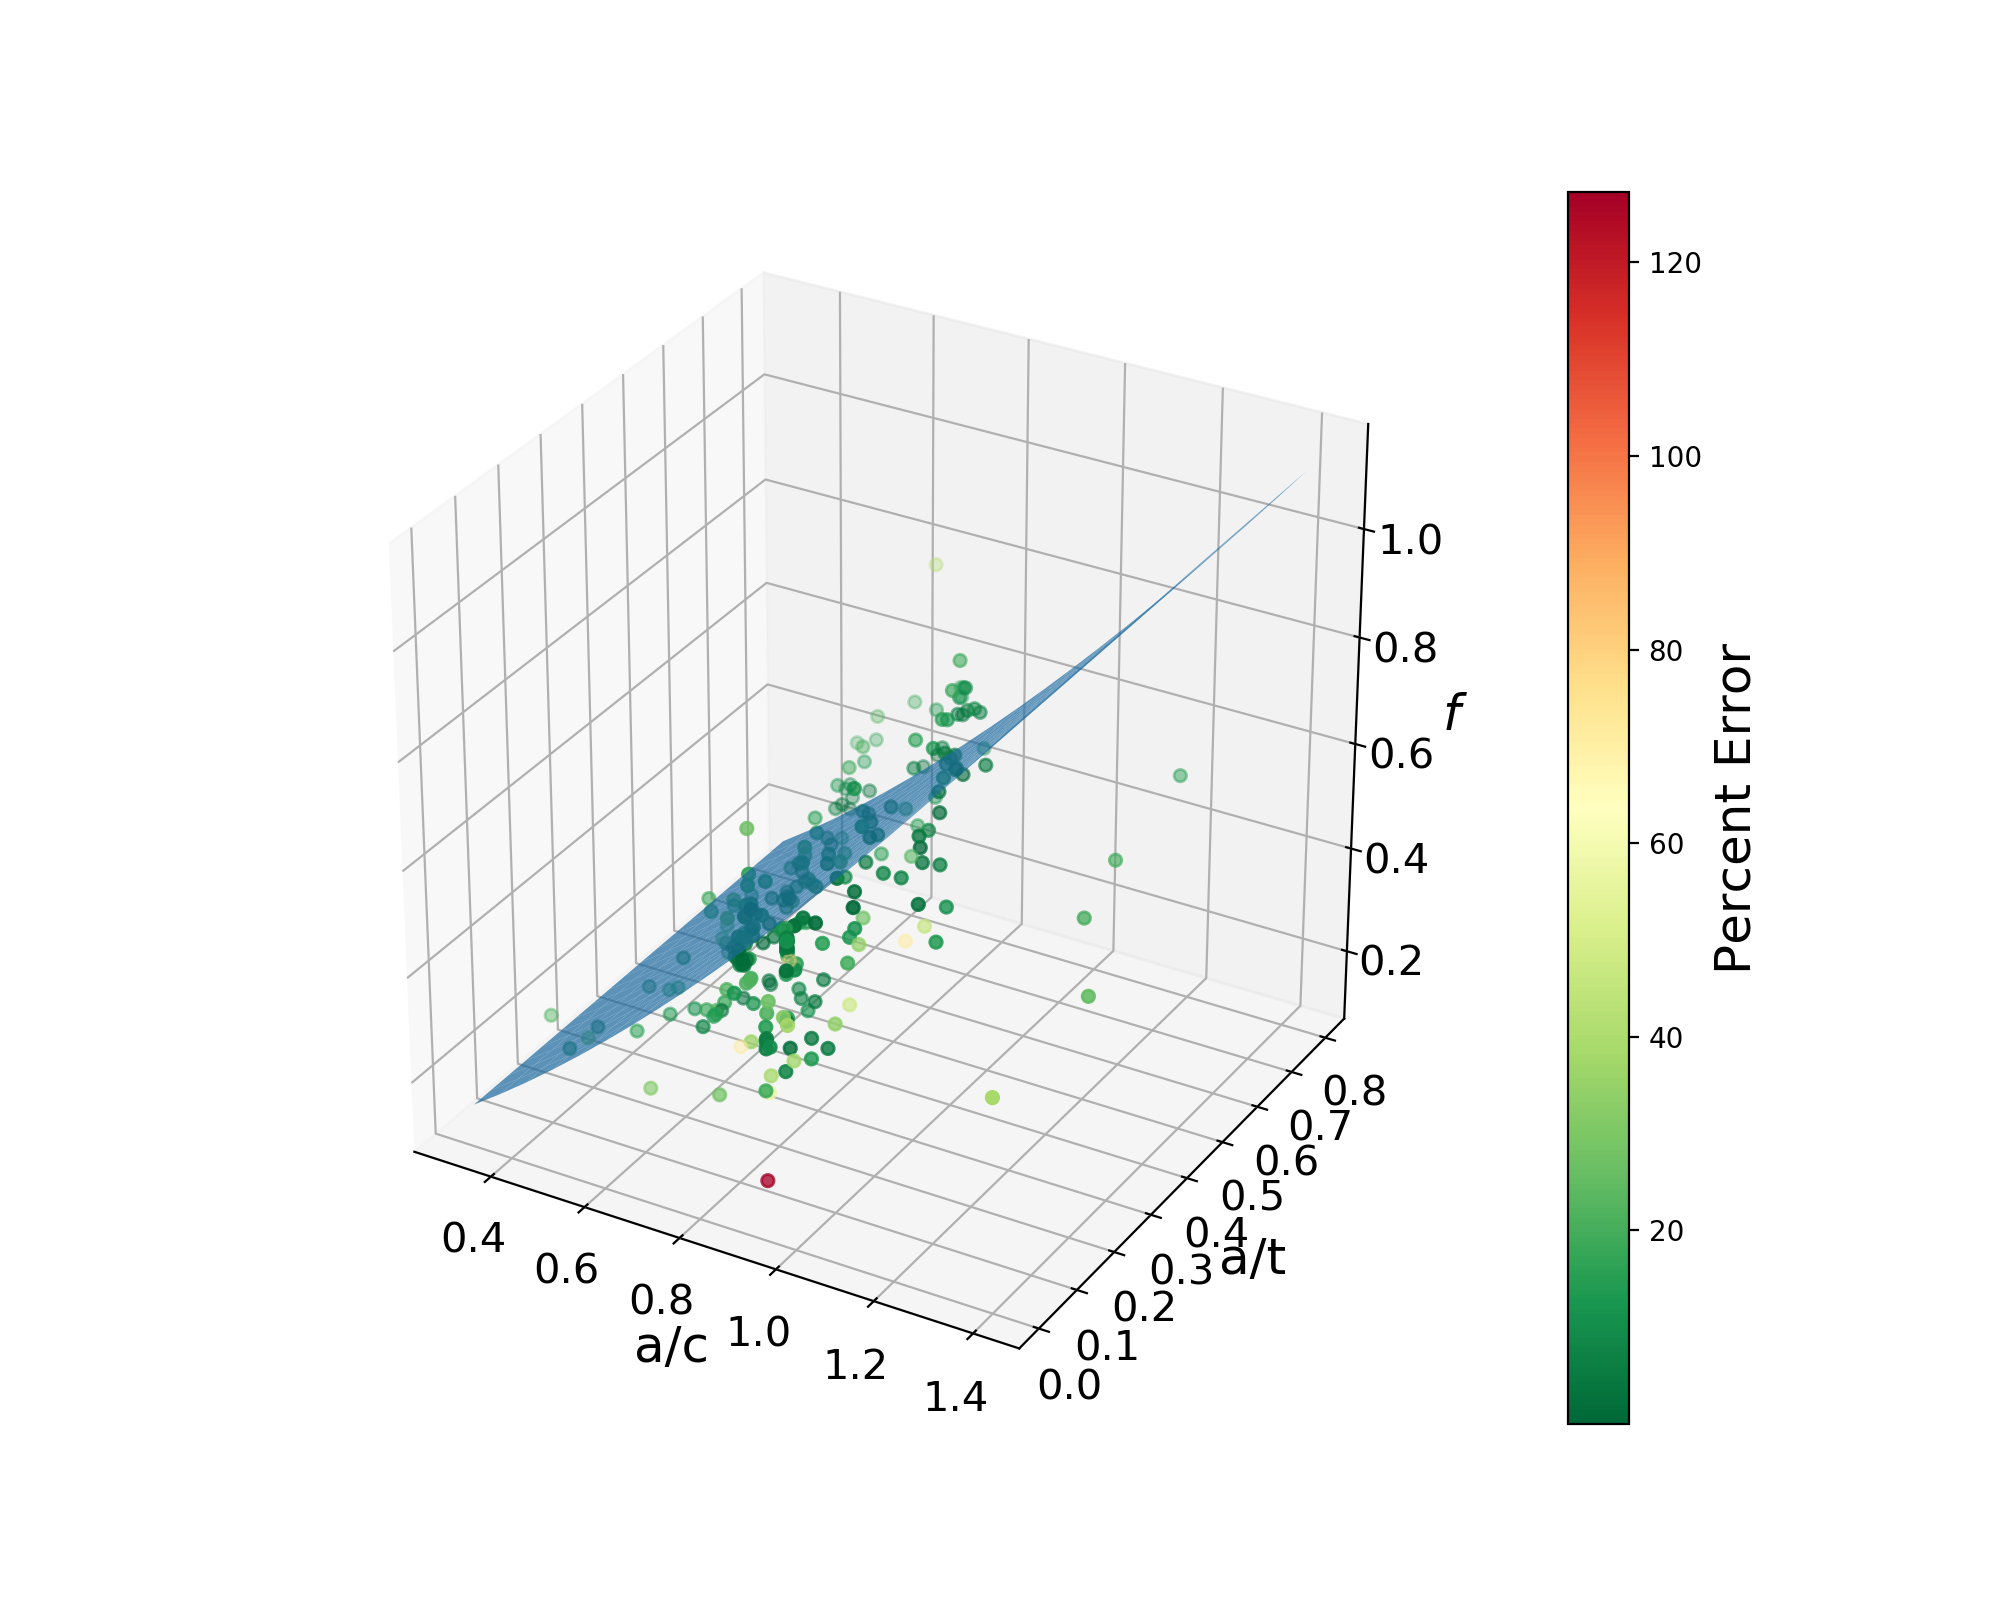
\includegraphics[width=\textwidth]{f1_surf.png}
    \caption{$f_1$ compared to the data}
    \label{fig:f1_surf}
  \end{subfigure}
  \hfill
  \begin{subfigure}[b]{0.5\textwidth}
    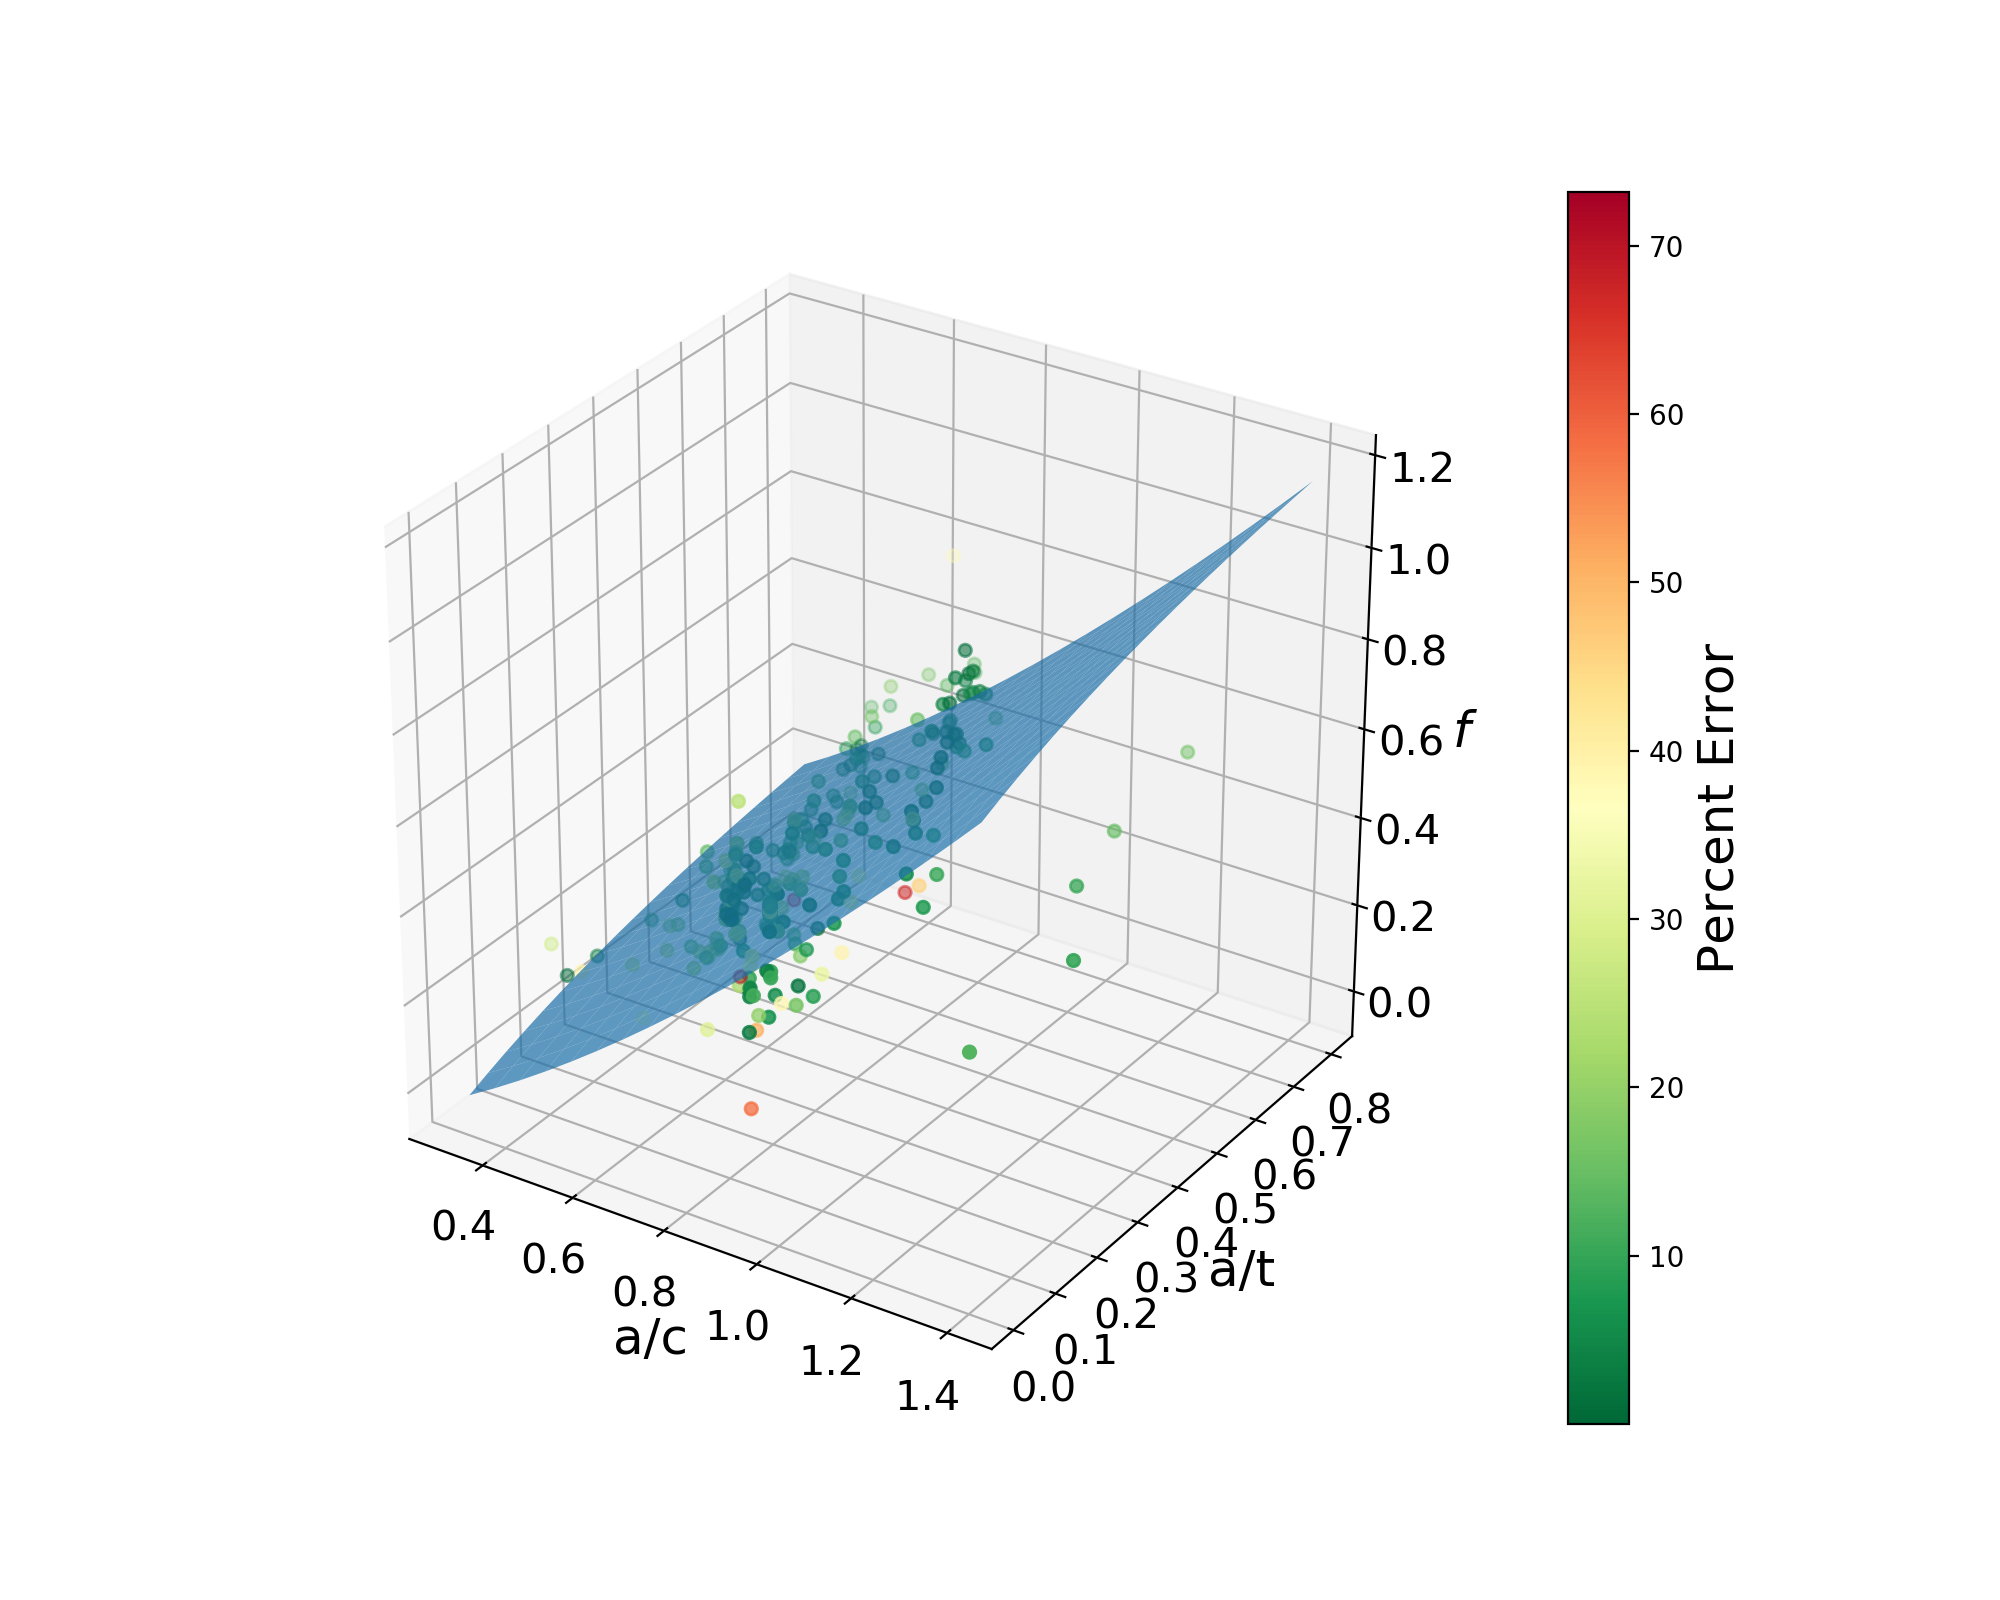
\includegraphics[width=\textwidth]{f1f2_surf.png}
    \caption{$f_1 + f^{'}_{2}$ compared to the data}
    \label{fig:f2_surf}
  \end{subfigure}
  \hfill
  \begin{subfigure}[b]{0.5\textwidth}
    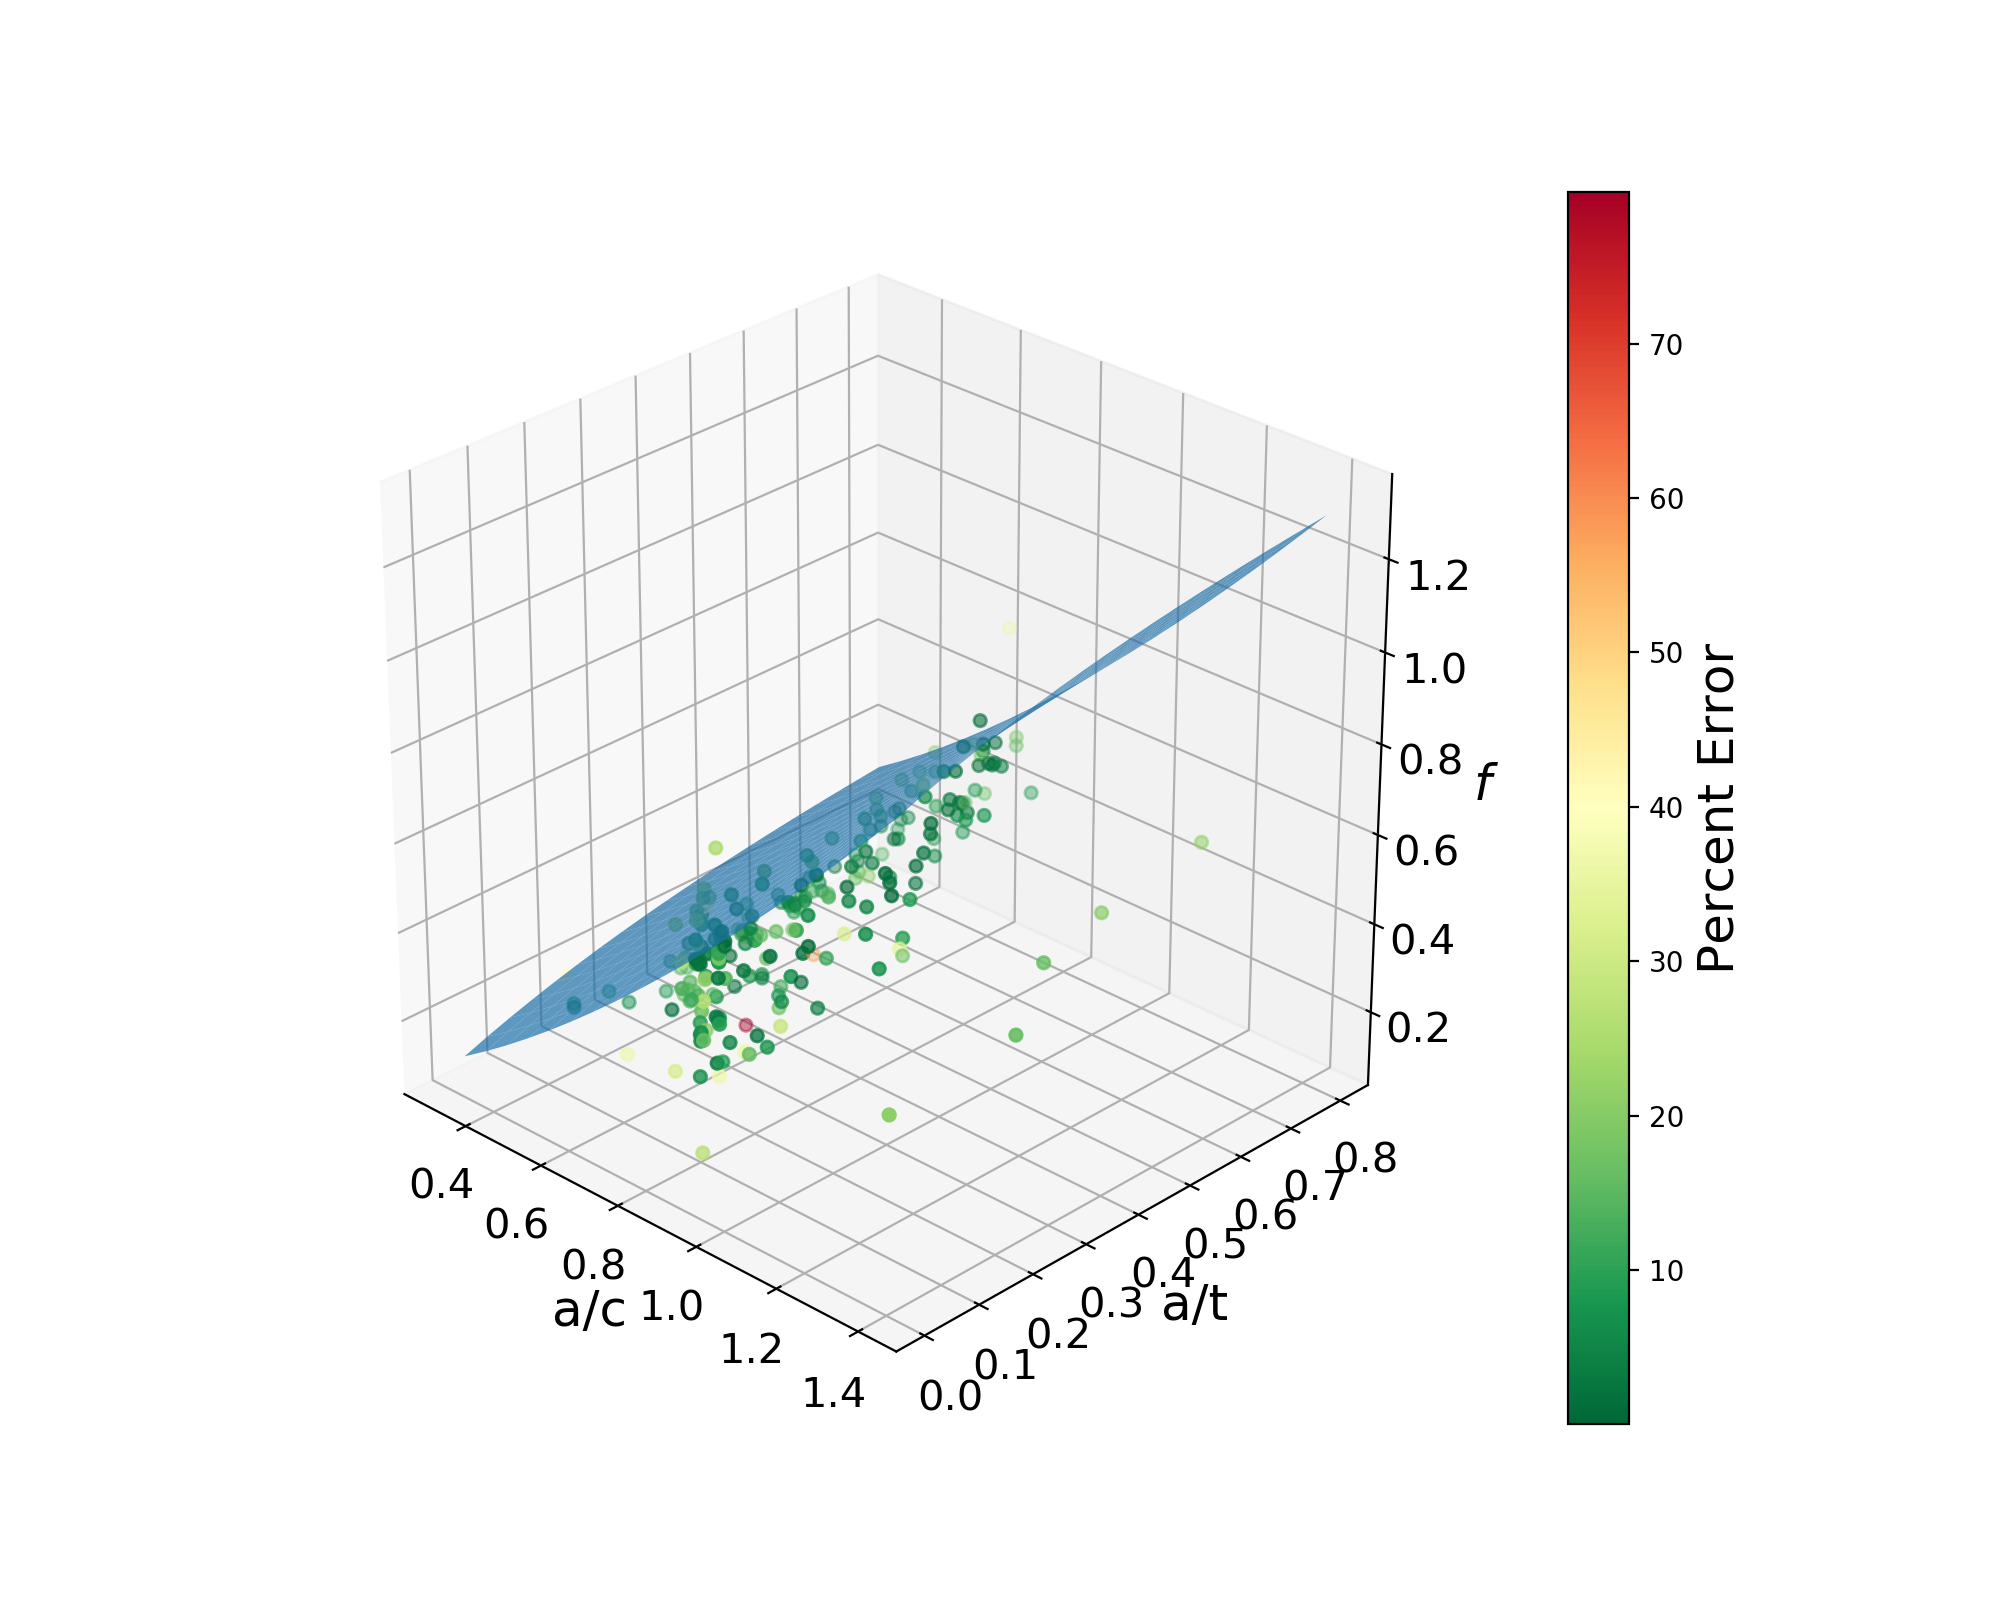
\includegraphics[width=\textwidth]{f1f2f3_surf.png}
    \caption{$f_1 + f^{'}_{2} + f_3$ compared to the data}
    \label{fig:f3_surf}
  \end{subfigure}
  \hfill
  \begin{subfigure}[b]{0.5\textwidth}
    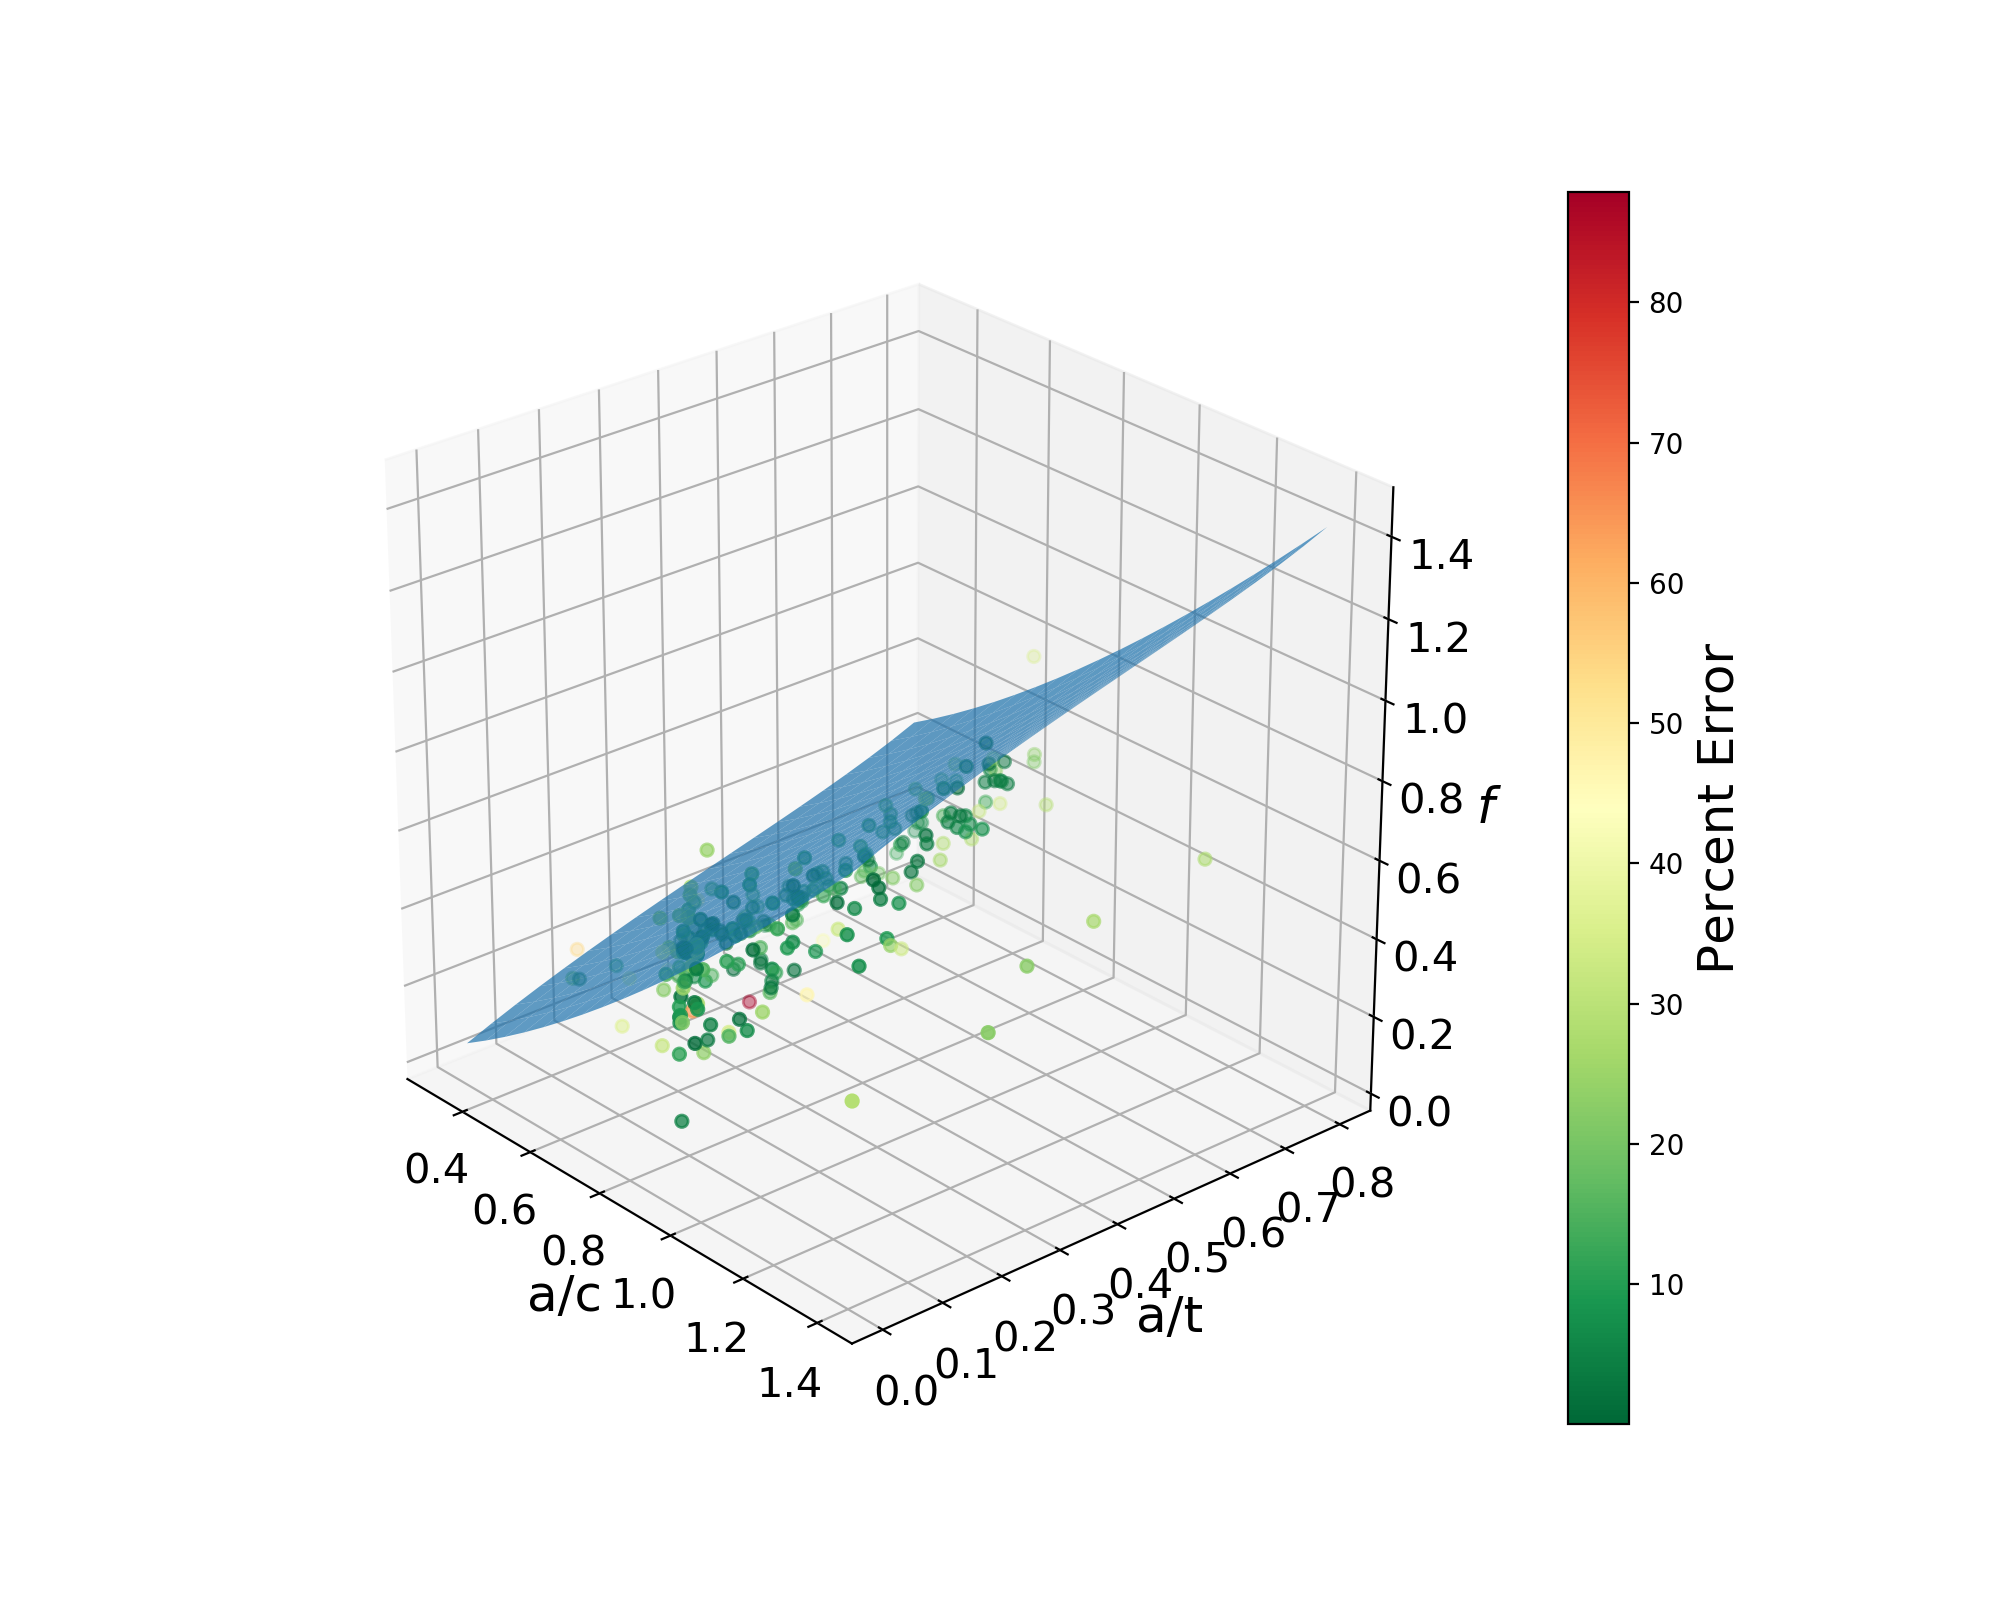
\includegraphics[width=\textwidth]{f1f2f3f4_surf.png}
    \caption{$f_1 + f^{'}_{2} + f_3 + f_4$ compared to the data}
    \label{fig:f4_surf}
  \end{subfigure}

  \caption{Three-dimensional slices of the six-dimensional data with
$\frac{a}{c}$ and $\frac{a}{t}$ as the displayed input variables of $f$ The
surfaces represents the functions.}

\end{figure}

%END OF CHAPTER TABLES

\begin{table}[h!]
\centering
\label{tab:max_disps}
\caption{\label{tab:max_disps}Maximum applied displacements of each boundary
condition such that displacement error between the structural- and solid-element
models remains below 1\%}

\begin{tabular}{ |c|c| } 
\hline
Disp. BC & Maximum displacement (mm) \\
\hline
z-displacement on surfaces 6 \& 60 & 0.03 \\ 
x-displacement on surface 3 & 0.01 \\ 
y-displacement on surfaces 4 \& 40 & 0.02\\ 
x-displacement on surface 4 & 0.03 \\ 
\hline
\end{tabular}
\end{table}

\begin{table}[h!]
\centering
\label{tab:sobol_indices}
\caption{\label{tab:sobol_indices}The first order and total sensitivity index as
defined by Sobol' for each displacement BC and their effect on maximum principal
stress as well as their confidence intervals.}
\begin{tabular}{ |c|c|c|c|c| } 
\hline
Disp. BC & S1 & 95\% CI & ST & 95\% CI \\
\hline
z-displacement on surfaces 6 \& 60 & 0.167 & 0.182 & 0.128 & 0.089 \\ 
x-displacement on surface 3 & 0.0145 & 0.312 & 0.239 & 0.334 \\ 
y-displacement on surfaces 4 \& 40 & 0.203 & 0.257 & 0.189 & 0.162 \\ 
x-displacement on surface 4 & 0.303 & 0.300 & 0.274 & 0.230 \\ 
\hline
\end{tabular}
\end{table}

\begin{table}[h!]
\centering
\label{tab:fitnesses}

\caption{\label{tab:fitnesses}Mean absolute error of each summed model including
the simplified model of $f_2$, $f^{'}_{2}$}

\begin{tabular}{ |c|c| } 
\hline
Summed Models & Mean Absolute Error \\
\hline
$f_1$ & 0.0543 \\ 
$f_1 + f_2$ & 0.0482 \\ 
$f_1 + f_2 + f_3$ & 0.0466 \\
$f_1 + f_2 + f_3 + f_3$ & 0.0570 \\
$f_1 + f^{'}_{2}$ & 0.0485 \\ 
$f_1 + f^{'}_{2} + f_3$ & 0.0468 \\
$f_1 + f^{'}_{2} + f_3 + f_3$ & 0.0570 \\
\hline
\end{tabular}
\end{table}